% **************************************************************************************************************
% A Classic Thesis Style
% An Homage to The Elements of Typographic Style
%
% Copyright (C) 2012 Andr\'e Miede http://www.miede.de
%
% If you like the style then I would appreciate a postcard. My address 
% can be found in the file ClassicThesis.pdf. A collection of the 
% postcards I received so far is available online at 
% http://postcards.miede.de
%
% License:
% This program is free software; you can redistribute it and/or modify
% it under the terms of the GNU General Public License as published by
% the Free Software Foundation; either version 2 of the License, or
% (at your option) any later version.
%
% This program is distributed in the hope that it will be useful,
% but WITHOUT ANY WARRANTY; without even the implied warranty of
% MERCHANTABILITY or FITNESS FOR A PARTICULAR PURPOSE.  See the
% GNU General Public License for more details.
%
% You should have received a copy of the GNU General Public License
% along with this program; see the file COPYING.  If not, write to
% the Free Software Foundation, Inc., 59 Temple Place - Suite 330,
% Boston, MA 02111-1307, USA.
%
% **************************************************************************************************************
% Note:
%    * You must not use "u etc. in strings/commands that will be spaced out (use \"u or real umlauts instead)
%    * New enumeration (small caps): \begin{aenumerate} \end{aenumerate}
%    * For margin notes: \marginpar or \graffito{}
%    * Do not use bold fonts in this style, it is designed around them
%    * Use tables as in the examples
%    * See classicthesis-preamble.sty for useful commands
% **************************************************************************************************************
% To Do:
%		 * [high] Check this out: http://www.golatex.de/koma-script-warnung-in-verbindung-mit-listings-package-t2058.html
%    * [medium] mathbb in section-titles/chapter-titles => disappears somehow in headlines!!!
% **************************************************************************************************************
\documentclass[ twoside,openright,titlepage,numbers=noenddot,headinclude,%1headlines,% letterpaper a4paper
                footinclude=true,cleardoublepage=empty,abstractoff, % <--- obsolete, remove (todo)
                BCOR=5mm,paper=a4,fontsize=11pt,%11pt,a4paper,%
                ngerman,american,%
                ]{scrreprt}

%********************************************************************
% Note: Make all your adjustments in here
%*******************************************************
% ****************************************************************************************************
% classicthesis-config.tex 
% formerly known as loadpackages.sty, classicthesis-ldpkg.sty, and classicthesis-preamble.sty 
% Use it at the beginning of your ClassicThesis.tex, or as a LaTeX Preamble 
% in your ClassicThesis.{tex,lyx} with % ****************************************************************************************************
% classicthesis-config.tex 
% formerly known as loadpackages.sty, classicthesis-ldpkg.sty, and classicthesis-preamble.sty 
% Use it at the beginning of your ClassicThesis.tex, or as a LaTeX Preamble 
% in your ClassicThesis.{tex,lyx} with % ****************************************************************************************************
% classicthesis-config.tex 
% formerly known as loadpackages.sty, classicthesis-ldpkg.sty, and classicthesis-preamble.sty 
% Use it at the beginning of your ClassicThesis.tex, or as a LaTeX Preamble 
% in your ClassicThesis.{tex,lyx} with \input{classicthesis-config}
% ****************************************************************************************************  
% If you like the classicthesis, then I would appreciate a postcard. 
% My address can be found in the file ClassicThesis.pdf. A collection 
% of the postcards I received so far is available online at 
% http://postcards.miede.de
% ****************************************************************************************************

% ****************************************************************************************************
% 1. Configure classicthesis for your needs here, e.g., remove "drafting" below 
% in order to deactivate the time-stamp on the pages
% ****************************************************************************************************
\PassOptionsToPackage{eulerchapternumbers,listings,%
				 pdfspacing,%floatperchapter,%linedheaders,%
				 subfig,beramono,eulermath,parts}{classicthesis}										
% ********************************************************************
% Available options for classicthesis.sty 
% (see ClassicThesis.pdf for more information):
% drafting
% parts nochapters linedheaders
% eulerchapternumbers beramono eulermath pdfspacing minionprospacing
% tocaligned dottedtoc manychapters
% listings floatperchapter subfig
% ********************************************************************

% ********************************************************************
% Triggers for this config
% ******************************************************************** 
\usepackage{ifthen}
\newboolean{enable-backrefs} % enable backrefs in the bibliography
\setboolean{enable-backrefs}{false} % true false
% ****************************************************************************************************


% ****************************************************************************************************
% 2. Personal data and user ad-hoc commands
% ****************************************************************************************************
\newcommand{\myTitle}{Meta Heuristic Extended Local Planning\xspace}
\newcommand{\mySubtitle}{}
\newcommand{\myDegree}{Doktor-Ingenieur (Dr.-Ing.)\xspace}
\newcommand{\myName}{Markus Suchi\xspace}
\newcommand{\myProf}{Put name here\xspace}
\newcommand{\myOtherProf}{Put name here\xspace}
\newcommand{\mySupervisor}{Put name here\xspace}
\newcommand{\myFaculty}{Put data here\xspace}
\newcommand{\myDepartment}{Put data here\xspace}
\newcommand{\myUni}{Put data here\xspace}
\newcommand{\myLocation}{Darmstadt\xspace}
\newcommand{\myTime}{August 2012\xspace}
\newcommand{\myVersion}{version 4.1\xspace}

% ********************************************************************
% Setup, finetuning, and useful commands
% ********************************************************************
\newcounter{dummy} % necessary for correct hyperlinks (to index, bib, etc.)
\newlength{\abcd} % for ab..z string length calculation
\providecommand{\mLyX}{L\kern-.1667em\lower.25em\hbox{Y}\kern-.125emX\@}
\newcommand{\ie}{i.\,e.}
\newcommand{\Ie}{I.\,e.}
\newcommand{\eg}{e.\,g.}
\newcommand{\Eg}{E.\,g.} 
% ****************************************************************************************************


% ****************************************************************************************************
% 3. Loading some handy packages
% ****************************************************************************************************
% ******************************************************************** 
% Packages with options that might require adjustments
% ******************************************************************** 
\PassOptionsToPackage{latin9}{inputenc}	% latin9 (ISO-8859-9) = latin1+"Euro sign"
 \usepackage{inputenc}				

%\PassOptionsToPackage{ngerman,american}{babel}   % change this to your language(s)
% Spanish languages need extra options in order to work with this template
%\PassOptionsToPackage{spanish,es-lcroman}{babel}
 \usepackage{babel}					

\PassOptionsToPackage{square,numbers}{natbib}
 \usepackage{natbib}				

\PassOptionsToPackage{fleqn}{amsmath}		% math environments and more by the AMS 
 \usepackage{amsmath}

% ******************************************************************** 
% General useful packages
% ******************************************************************** 
\usepackage[ ]{pdfpages}

\PassOptionsToPackage{T1}{fontenc} % T2A for cyrillics
	\usepackage{fontenc}     
\usepackage{textcomp} % fix warning with missing font shapes
\usepackage{scrhack} % fix warnings when using KOMA with listings package          
\usepackage{xspace} % to get the spacing after macros right  
\usepackage{mparhack} % get marginpar right
\usepackage{fixltx2e} % fixes some LaTeX stuff 
\PassOptionsToPackage{printonlyused,smaller}{acronym}
	\usepackage{acronym} % nice macros for handling all acronyms in the thesis
%\renewcommand*{\acsfont}[1]{\textssc{#1}} % for MinionPro
\renewcommand{\bflabel}[1]{{#1}\hfill} % fix the list of acronyms
% ****************************************************************************************************


% ****************************************************************************************************
% 4. Setup floats: tables, (sub)figures, and captions
% ****************************************************************************************************
\usepackage{tabularx} % better tables
	\setlength{\extrarowheight}{3pt} % increase table row height
\newcommand{\tableheadline}[1]{\multicolumn{1}{c}{\spacedlowsmallcaps{#1}}}
\newcommand{\myfloatalign}{\centering} % to be used with each float for alignment
\usepackage{caption}
\captionsetup{format=hang,font=small}
\usepackage{subfig}  
% ****************************************************************************************************


% ****************************************************************************************************
% 5. Setup code listings
% ****************************************************************************************************
\usepackage{listings} 
%\lstset{emph={trueIndex,root},emphstyle=\color{BlueViolet}}%\underbar} % for special keywords
\lstset{language=[LaTeX]Tex,%C++,
    keywordstyle=\color{RoyalBlue},%\bfseries,
    basicstyle=\small\ttfamily,
    %identifierstyle=\color{NavyBlue},
    commentstyle=\color{Green}\ttfamily,
    stringstyle=\rmfamily,
    numbers=none,%left,%
    numberstyle=\scriptsize,%\tiny
    stepnumber=5,
    numbersep=8pt,
    showstringspaces=false,
    breaklines=true,
    frameround=ftff,
    frame=single,
    belowcaptionskip=.75\baselineskip
    %frame=L
} 
% ****************************************************************************************************    		   


% ****************************************************************************************************
% 6. PDFLaTeX, hyperreferences and citation backreferences
% ****************************************************************************************************
% ********************************************************************
% Using PDFLaTeX
% ********************************************************************
\PassOptionsToPackage{pdftex,hyperfootnotes=false,pdfpagelabels}{hyperref}
	\usepackage{hyperref}  % backref linktocpage pagebackref
\pdfcompresslevel=9
\pdfadjustspacing=1 
\PassOptionsToPackage{pdftex}{graphicx}
	\usepackage{graphicx} 

% ********************************************************************
% Setup the style of the backrefs from the bibliography
% (translate the options to any language you use)
% ********************************************************************
\newcommand{\backrefnotcitedstring}{\relax}%(Not cited.)
\newcommand{\backrefcitedsinglestring}[1]{(Cited on page~#1.)}
\newcommand{\backrefcitedmultistring}[1]{(Cited on pages~#1.)}
\ifthenelse{\boolean{enable-backrefs}}%
{%
		\PassOptionsToPackage{hyperpageref}{backref}
		\usepackage{backref} % to be loaded after hyperref package 
		   \renewcommand{\backreftwosep}{ and~} % separate 2 pages
		   \renewcommand{\backreflastsep}{, and~} % separate last of longer list
		   \renewcommand*{\backref}[1]{}  % disable standard
		   \renewcommand*{\backrefalt}[4]{% detailed backref
		      \ifcase #1 %
		         \backrefnotcitedstring%
		      \or%
		         \backrefcitedsinglestring{#2}%
		      \else%
		         \backrefcitedmultistring{#2}%
		      \fi}%
}{\relax}    

% ********************************************************************
% Hyperreferences
% ********************************************************************
\hypersetup{%
    %draft,	% = no hyperlinking at all (useful in b/w printouts)
    colorlinks=true, linktocpage=true, pdfstartpage=3, pdfstartview=FitV,%
    % uncomment the following line if you want to have black links (e.g., for printing)
    %colorlinks=false, linktocpage=false, pdfborder={0 0 0}, pdfstartpage=3, pdfstartview=FitV,% 
    breaklinks=true, pdfpagemode=UseNone, pageanchor=true, pdfpagemode=UseOutlines,%
    plainpages=false, bookmarksnumbered, bookmarksopen=true, bookmarksopenlevel=1,%
    hypertexnames=true, pdfhighlight=/O,%nesting=true,%frenchlinks,%
    urlcolor=webbrown, linkcolor=RoyalBlue, citecolor=webgreen, %pagecolor=RoyalBlue,%
    %urlcolor=Black, linkcolor=Black, citecolor=Black, %pagecolor=Black,%
    pdftitle={\myTitle},%
    pdfauthor={\textcopyright\ \myName, \myUni, \myFaculty},%
    pdfsubject={},%
    pdfkeywords={},%
    pdfcreator={pdfLaTeX},%
    pdfproducer={LaTeX with hyperref and classicthesis}%
}   

% ********************************************************************
% Setup autoreferences
% ********************************************************************
% There are some issues regarding autorefnames
% http://www.ureader.de/msg/136221647.aspx
% http://www.tex.ac.uk/cgi-bin/texfaq2html?label=latexwords
% you have to redefine the makros for the 
% language you use, e.g., american, ngerman
% (as chosen when loading babel/AtBeginDocument)
% ********************************************************************
\makeatletter
\@ifpackageloaded{babel}%
    {%
       \addto\extrasamerican{%
					\renewcommand*{\figureautorefname}{Figure}%
					\renewcommand*{\tableautorefname}{Table}%
					\renewcommand*{\partautorefname}{Part}%
					\renewcommand*{\chapterautorefname}{Chapter}%
					\renewcommand*{\sectionautorefname}{Section}%
					\renewcommand*{\subsectionautorefname}{Section}%
					\renewcommand*{\subsubsectionautorefname}{Section}% 	
				}%
       \addto\extrasngerman{% 
					\renewcommand*{\paragraphautorefname}{Absatz}%
					\renewcommand*{\subparagraphautorefname}{Unterabsatz}%
					\renewcommand*{\footnoteautorefname}{Fu\"snote}%
					\renewcommand*{\FancyVerbLineautorefname}{Zeile}%
					\renewcommand*{\theoremautorefname}{Theorem}%
					\renewcommand*{\appendixautorefname}{Anhang}%
					\renewcommand*{\equationautorefname}{Gleichung}%        
					\renewcommand*{\itemautorefname}{Punkt}%
				}%	
			% Fix to getting autorefs for subfigures right (thanks to Belinda Vogt for changing the definition)
			\providecommand{\subfigureautorefname}{\figureautorefname}%  			
    }{\relax}
\makeatother


% ****************************************************************************************************
% 7. Last calls before the bar closes
% ****************************************************************************************************
% ********************************************************************
% Development Stuff
% ********************************************************************
\listfiles
%\PassOptionsToPackage{l2tabu,orthodox,abort}{nag}
%	\usepackage{nag}
%\PassOptionsToPackage{warning, all}{onlyamsmath}
%	\usepackage{onlyamsmath}

% ********************************************************************
% Last, but not least...
% ********************************************************************
\usepackage{classicthesis} 
% ****************************************************************************************************


% ****************************************************************************************************
% 8. Further adjustments (experimental)
% ****************************************************************************************************
% ********************************************************************
% Changing the text area
% ********************************************************************
%\linespread{1.05} % a bit more for Palatino
%\areaset[current]{312pt}{761pt} % 686 (factor 2.2) + 33 head + 42 head \the\footskip
%\setlength{\marginparwidth}{7em}%
%\setlength{\marginparsep}{2em}%

% ********************************************************************
% Using different fonts
% ********************************************************************
%\usepackage[oldstylenums]{kpfonts} % oldstyle notextcomp
%\usepackage[osf]{libertine}
%\usepackage{hfoldsty} % Computer Modern with osf
%\usepackage[light,condensed,math]{iwona}
%\renewcommand{\sfdefault}{iwona}
%\usepackage{lmodern} % <-- no osf support :-(
%\usepackage[urw-garamond]{mathdesign} <-- no osf support :-(
% ****************************************************************************************************

\usepackage[lined,linesnumbered,algochapter]{algorithm} % Algorithm-Environment
\usepackage{algpseudocode} % Algorithm-Environment

\graphicspath{{figures/}{figures/titlepage/}} 
\usepackage{calc}
\newcommand{\executeiffilenewer}[3]{%
 \ifnum\pdfstrcmp{\pdffilemoddate{#1}}%
 {\pdffilemoddate{#2}}>0%
 {\immediate\write18{#3}}\fi%
}

\newcommand{\includesvg}[1]{%
 \executeiffilenewer{#1.svg}{figures/#1.pdf}%
 {inkscape -z --file=#1.svg %
 --export-pdf=#1.pdf --export-latex}%
 \input{#1.pdf_tex}%
}
% ****************************************************************************************************  
% If you like the classicthesis, then I would appreciate a postcard. 
% My address can be found in the file ClassicThesis.pdf. A collection 
% of the postcards I received so far is available online at 
% http://postcards.miede.de
% ****************************************************************************************************

% ****************************************************************************************************
% 1. Configure classicthesis for your needs here, e.g., remove "drafting" below 
% in order to deactivate the time-stamp on the pages
% ****************************************************************************************************
\PassOptionsToPackage{eulerchapternumbers,listings,%
				 pdfspacing,%floatperchapter,%linedheaders,%
				 subfig,beramono,eulermath,parts}{classicthesis}										
% ********************************************************************
% Available options for classicthesis.sty 
% (see ClassicThesis.pdf for more information):
% drafting
% parts nochapters linedheaders
% eulerchapternumbers beramono eulermath pdfspacing minionprospacing
% tocaligned dottedtoc manychapters
% listings floatperchapter subfig
% ********************************************************************

% ********************************************************************
% Triggers for this config
% ******************************************************************** 
\usepackage{ifthen}
\newboolean{enable-backrefs} % enable backrefs in the bibliography
\setboolean{enable-backrefs}{false} % true false
% ****************************************************************************************************


% ****************************************************************************************************
% 2. Personal data and user ad-hoc commands
% ****************************************************************************************************
\newcommand{\myTitle}{Meta Heuristic Extended Local Planning\xspace}
\newcommand{\mySubtitle}{}
\newcommand{\myDegree}{Doktor-Ingenieur (Dr.-Ing.)\xspace}
\newcommand{\myName}{Markus Suchi\xspace}
\newcommand{\myProf}{Put name here\xspace}
\newcommand{\myOtherProf}{Put name here\xspace}
\newcommand{\mySupervisor}{Put name here\xspace}
\newcommand{\myFaculty}{Put data here\xspace}
\newcommand{\myDepartment}{Put data here\xspace}
\newcommand{\myUni}{Put data here\xspace}
\newcommand{\myLocation}{Darmstadt\xspace}
\newcommand{\myTime}{August 2012\xspace}
\newcommand{\myVersion}{version 4.1\xspace}

% ********************************************************************
% Setup, finetuning, and useful commands
% ********************************************************************
\newcounter{dummy} % necessary for correct hyperlinks (to index, bib, etc.)
\newlength{\abcd} % for ab..z string length calculation
\providecommand{\mLyX}{L\kern-.1667em\lower.25em\hbox{Y}\kern-.125emX\@}
\newcommand{\ie}{i.\,e.}
\newcommand{\Ie}{I.\,e.}
\newcommand{\eg}{e.\,g.}
\newcommand{\Eg}{E.\,g.} 
% ****************************************************************************************************


% ****************************************************************************************************
% 3. Loading some handy packages
% ****************************************************************************************************
% ******************************************************************** 
% Packages with options that might require adjustments
% ******************************************************************** 
\PassOptionsToPackage{latin9}{inputenc}	% latin9 (ISO-8859-9) = latin1+"Euro sign"
 \usepackage{inputenc}				

%\PassOptionsToPackage{ngerman,american}{babel}   % change this to your language(s)
% Spanish languages need extra options in order to work with this template
%\PassOptionsToPackage{spanish,es-lcroman}{babel}
 \usepackage{babel}					

\PassOptionsToPackage{square,numbers}{natbib}
 \usepackage{natbib}				

\PassOptionsToPackage{fleqn}{amsmath}		% math environments and more by the AMS 
 \usepackage{amsmath}

% ******************************************************************** 
% General useful packages
% ******************************************************************** 
\usepackage[ ]{pdfpages}

\PassOptionsToPackage{T1}{fontenc} % T2A for cyrillics
	\usepackage{fontenc}     
\usepackage{textcomp} % fix warning with missing font shapes
\usepackage{scrhack} % fix warnings when using KOMA with listings package          
\usepackage{xspace} % to get the spacing after macros right  
\usepackage{mparhack} % get marginpar right
\usepackage{fixltx2e} % fixes some LaTeX stuff 
\PassOptionsToPackage{printonlyused,smaller}{acronym}
	\usepackage{acronym} % nice macros for handling all acronyms in the thesis
%\renewcommand*{\acsfont}[1]{\textssc{#1}} % for MinionPro
\renewcommand{\bflabel}[1]{{#1}\hfill} % fix the list of acronyms
% ****************************************************************************************************


% ****************************************************************************************************
% 4. Setup floats: tables, (sub)figures, and captions
% ****************************************************************************************************
\usepackage{tabularx} % better tables
	\setlength{\extrarowheight}{3pt} % increase table row height
\newcommand{\tableheadline}[1]{\multicolumn{1}{c}{\spacedlowsmallcaps{#1}}}
\newcommand{\myfloatalign}{\centering} % to be used with each float for alignment
\usepackage{caption}
\captionsetup{format=hang,font=small}
\usepackage{subfig}  
% ****************************************************************************************************


% ****************************************************************************************************
% 5. Setup code listings
% ****************************************************************************************************
\usepackage{listings} 
%\lstset{emph={trueIndex,root},emphstyle=\color{BlueViolet}}%\underbar} % for special keywords
\lstset{language=[LaTeX]Tex,%C++,
    keywordstyle=\color{RoyalBlue},%\bfseries,
    basicstyle=\small\ttfamily,
    %identifierstyle=\color{NavyBlue},
    commentstyle=\color{Green}\ttfamily,
    stringstyle=\rmfamily,
    numbers=none,%left,%
    numberstyle=\scriptsize,%\tiny
    stepnumber=5,
    numbersep=8pt,
    showstringspaces=false,
    breaklines=true,
    frameround=ftff,
    frame=single,
    belowcaptionskip=.75\baselineskip
    %frame=L
} 
% ****************************************************************************************************    		   


% ****************************************************************************************************
% 6. PDFLaTeX, hyperreferences and citation backreferences
% ****************************************************************************************************
% ********************************************************************
% Using PDFLaTeX
% ********************************************************************
\PassOptionsToPackage{pdftex,hyperfootnotes=false,pdfpagelabels}{hyperref}
	\usepackage{hyperref}  % backref linktocpage pagebackref
\pdfcompresslevel=9
\pdfadjustspacing=1 
\PassOptionsToPackage{pdftex}{graphicx}
	\usepackage{graphicx} 

% ********************************************************************
% Setup the style of the backrefs from the bibliography
% (translate the options to any language you use)
% ********************************************************************
\newcommand{\backrefnotcitedstring}{\relax}%(Not cited.)
\newcommand{\backrefcitedsinglestring}[1]{(Cited on page~#1.)}
\newcommand{\backrefcitedmultistring}[1]{(Cited on pages~#1.)}
\ifthenelse{\boolean{enable-backrefs}}%
{%
		\PassOptionsToPackage{hyperpageref}{backref}
		\usepackage{backref} % to be loaded after hyperref package 
		   \renewcommand{\backreftwosep}{ and~} % separate 2 pages
		   \renewcommand{\backreflastsep}{, and~} % separate last of longer list
		   \renewcommand*{\backref}[1]{}  % disable standard
		   \renewcommand*{\backrefalt}[4]{% detailed backref
		      \ifcase #1 %
		         \backrefnotcitedstring%
		      \or%
		         \backrefcitedsinglestring{#2}%
		      \else%
		         \backrefcitedmultistring{#2}%
		      \fi}%
}{\relax}    

% ********************************************************************
% Hyperreferences
% ********************************************************************
\hypersetup{%
    %draft,	% = no hyperlinking at all (useful in b/w printouts)
    colorlinks=true, linktocpage=true, pdfstartpage=3, pdfstartview=FitV,%
    % uncomment the following line if you want to have black links (e.g., for printing)
    %colorlinks=false, linktocpage=false, pdfborder={0 0 0}, pdfstartpage=3, pdfstartview=FitV,% 
    breaklinks=true, pdfpagemode=UseNone, pageanchor=true, pdfpagemode=UseOutlines,%
    plainpages=false, bookmarksnumbered, bookmarksopen=true, bookmarksopenlevel=1,%
    hypertexnames=true, pdfhighlight=/O,%nesting=true,%frenchlinks,%
    urlcolor=webbrown, linkcolor=RoyalBlue, citecolor=webgreen, %pagecolor=RoyalBlue,%
    %urlcolor=Black, linkcolor=Black, citecolor=Black, %pagecolor=Black,%
    pdftitle={\myTitle},%
    pdfauthor={\textcopyright\ \myName, \myUni, \myFaculty},%
    pdfsubject={},%
    pdfkeywords={},%
    pdfcreator={pdfLaTeX},%
    pdfproducer={LaTeX with hyperref and classicthesis}%
}   

% ********************************************************************
% Setup autoreferences
% ********************************************************************
% There are some issues regarding autorefnames
% http://www.ureader.de/msg/136221647.aspx
% http://www.tex.ac.uk/cgi-bin/texfaq2html?label=latexwords
% you have to redefine the makros for the 
% language you use, e.g., american, ngerman
% (as chosen when loading babel/AtBeginDocument)
% ********************************************************************
\makeatletter
\@ifpackageloaded{babel}%
    {%
       \addto\extrasamerican{%
					\renewcommand*{\figureautorefname}{Figure}%
					\renewcommand*{\tableautorefname}{Table}%
					\renewcommand*{\partautorefname}{Part}%
					\renewcommand*{\chapterautorefname}{Chapter}%
					\renewcommand*{\sectionautorefname}{Section}%
					\renewcommand*{\subsectionautorefname}{Section}%
					\renewcommand*{\subsubsectionautorefname}{Section}% 	
				}%
       \addto\extrasngerman{% 
					\renewcommand*{\paragraphautorefname}{Absatz}%
					\renewcommand*{\subparagraphautorefname}{Unterabsatz}%
					\renewcommand*{\footnoteautorefname}{Fu\"snote}%
					\renewcommand*{\FancyVerbLineautorefname}{Zeile}%
					\renewcommand*{\theoremautorefname}{Theorem}%
					\renewcommand*{\appendixautorefname}{Anhang}%
					\renewcommand*{\equationautorefname}{Gleichung}%        
					\renewcommand*{\itemautorefname}{Punkt}%
				}%	
			% Fix to getting autorefs for subfigures right (thanks to Belinda Vogt for changing the definition)
			\providecommand{\subfigureautorefname}{\figureautorefname}%  			
    }{\relax}
\makeatother


% ****************************************************************************************************
% 7. Last calls before the bar closes
% ****************************************************************************************************
% ********************************************************************
% Development Stuff
% ********************************************************************
\listfiles
%\PassOptionsToPackage{l2tabu,orthodox,abort}{nag}
%	\usepackage{nag}
%\PassOptionsToPackage{warning, all}{onlyamsmath}
%	\usepackage{onlyamsmath}

% ********************************************************************
% Last, but not least...
% ********************************************************************
\usepackage{classicthesis} 
% ****************************************************************************************************


% ****************************************************************************************************
% 8. Further adjustments (experimental)
% ****************************************************************************************************
% ********************************************************************
% Changing the text area
% ********************************************************************
%\linespread{1.05} % a bit more for Palatino
%\areaset[current]{312pt}{761pt} % 686 (factor 2.2) + 33 head + 42 head \the\footskip
%\setlength{\marginparwidth}{7em}%
%\setlength{\marginparsep}{2em}%

% ********************************************************************
% Using different fonts
% ********************************************************************
%\usepackage[oldstylenums]{kpfonts} % oldstyle notextcomp
%\usepackage[osf]{libertine}
%\usepackage{hfoldsty} % Computer Modern with osf
%\usepackage[light,condensed,math]{iwona}
%\renewcommand{\sfdefault}{iwona}
%\usepackage{lmodern} % <-- no osf support :-(
%\usepackage[urw-garamond]{mathdesign} <-- no osf support :-(
% ****************************************************************************************************

\usepackage[lined,linesnumbered,algochapter]{algorithm} % Algorithm-Environment
\usepackage{algpseudocode} % Algorithm-Environment

\graphicspath{{figures/}{figures/titlepage/}} 
\usepackage{calc}
\newcommand{\executeiffilenewer}[3]{%
 \ifnum\pdfstrcmp{\pdffilemoddate{#1}}%
 {\pdffilemoddate{#2}}>0%
 {\immediate\write18{#3}}\fi%
}

\newcommand{\includesvg}[1]{%
 \executeiffilenewer{#1.svg}{figures/#1.pdf}%
 {inkscape -z --file=#1.svg %
 --export-pdf=#1.pdf --export-latex}%
 \input{#1.pdf_tex}%
}
% ****************************************************************************************************  
% If you like the classicthesis, then I would appreciate a postcard. 
% My address can be found in the file ClassicThesis.pdf. A collection 
% of the postcards I received so far is available online at 
% http://postcards.miede.de
% ****************************************************************************************************

% ****************************************************************************************************
% 1. Configure classicthesis for your needs here, e.g., remove "drafting" below 
% in order to deactivate the time-stamp on the pages
% ****************************************************************************************************
\PassOptionsToPackage{eulerchapternumbers,listings,%
				 pdfspacing,%floatperchapter,%linedheaders,%
				 subfig,beramono,eulermath,parts}{classicthesis}										
% ********************************************************************
% Available options for classicthesis.sty 
% (see ClassicThesis.pdf for more information):
% drafting
% parts nochapters linedheaders
% eulerchapternumbers beramono eulermath pdfspacing minionprospacing
% tocaligned dottedtoc manychapters
% listings floatperchapter subfig
% ********************************************************************

% ********************************************************************
% Triggers for this config
% ******************************************************************** 
\usepackage{ifthen}
\newboolean{enable-backrefs} % enable backrefs in the bibliography
\setboolean{enable-backrefs}{false} % true false
% ****************************************************************************************************


% ****************************************************************************************************
% 2. Personal data and user ad-hoc commands
% ****************************************************************************************************
\newcommand{\myTitle}{Meta Heuristic Extended Local Planning\xspace}
\newcommand{\mySubtitle}{}
\newcommand{\myDegree}{Doktor-Ingenieur (Dr.-Ing.)\xspace}
\newcommand{\myName}{Markus Suchi\xspace}
\newcommand{\myProf}{Put name here\xspace}
\newcommand{\myOtherProf}{Put name here\xspace}
\newcommand{\mySupervisor}{Put name here\xspace}
\newcommand{\myFaculty}{Put data here\xspace}
\newcommand{\myDepartment}{Put data here\xspace}
\newcommand{\myUni}{Put data here\xspace}
\newcommand{\myLocation}{Darmstadt\xspace}
\newcommand{\myTime}{August 2012\xspace}
\newcommand{\myVersion}{version 4.1\xspace}

% ********************************************************************
% Setup, finetuning, and useful commands
% ********************************************************************
\newcounter{dummy} % necessary for correct hyperlinks (to index, bib, etc.)
\newlength{\abcd} % for ab..z string length calculation
\providecommand{\mLyX}{L\kern-.1667em\lower.25em\hbox{Y}\kern-.125emX\@}
\newcommand{\ie}{i.\,e.}
\newcommand{\Ie}{I.\,e.}
\newcommand{\eg}{e.\,g.}
\newcommand{\Eg}{E.\,g.} 
% ****************************************************************************************************


% ****************************************************************************************************
% 3. Loading some handy packages
% ****************************************************************************************************
% ******************************************************************** 
% Packages with options that might require adjustments
% ******************************************************************** 
\PassOptionsToPackage{latin9}{inputenc}	% latin9 (ISO-8859-9) = latin1+"Euro sign"
 \usepackage{inputenc}				

%\PassOptionsToPackage{ngerman,american}{babel}   % change this to your language(s)
% Spanish languages need extra options in order to work with this template
%\PassOptionsToPackage{spanish,es-lcroman}{babel}
 \usepackage{babel}					

\PassOptionsToPackage{square,numbers}{natbib}
 \usepackage{natbib}				

\PassOptionsToPackage{fleqn}{amsmath}		% math environments and more by the AMS 
 \usepackage{amsmath}

% ******************************************************************** 
% General useful packages
% ******************************************************************** 
\usepackage[ ]{pdfpages}

\PassOptionsToPackage{T1}{fontenc} % T2A for cyrillics
	\usepackage{fontenc}     
\usepackage{textcomp} % fix warning with missing font shapes
\usepackage{scrhack} % fix warnings when using KOMA with listings package          
\usepackage{xspace} % to get the spacing after macros right  
\usepackage{mparhack} % get marginpar right
\usepackage{fixltx2e} % fixes some LaTeX stuff 
\PassOptionsToPackage{printonlyused,smaller}{acronym}
	\usepackage{acronym} % nice macros for handling all acronyms in the thesis
%\renewcommand*{\acsfont}[1]{\textssc{#1}} % for MinionPro
\renewcommand{\bflabel}[1]{{#1}\hfill} % fix the list of acronyms
% ****************************************************************************************************


% ****************************************************************************************************
% 4. Setup floats: tables, (sub)figures, and captions
% ****************************************************************************************************
\usepackage{tabularx} % better tables
	\setlength{\extrarowheight}{3pt} % increase table row height
\newcommand{\tableheadline}[1]{\multicolumn{1}{c}{\spacedlowsmallcaps{#1}}}
\newcommand{\myfloatalign}{\centering} % to be used with each float for alignment
\usepackage{caption}
\captionsetup{format=hang,font=small}
\usepackage{subfig}  
% ****************************************************************************************************


% ****************************************************************************************************
% 5. Setup code listings
% ****************************************************************************************************
\usepackage{listings} 
%\lstset{emph={trueIndex,root},emphstyle=\color{BlueViolet}}%\underbar} % for special keywords
\lstset{language=[LaTeX]Tex,%C++,
    keywordstyle=\color{RoyalBlue},%\bfseries,
    basicstyle=\small\ttfamily,
    %identifierstyle=\color{NavyBlue},
    commentstyle=\color{Green}\ttfamily,
    stringstyle=\rmfamily,
    numbers=none,%left,%
    numberstyle=\scriptsize,%\tiny
    stepnumber=5,
    numbersep=8pt,
    showstringspaces=false,
    breaklines=true,
    frameround=ftff,
    frame=single,
    belowcaptionskip=.75\baselineskip
    %frame=L
} 
% ****************************************************************************************************    		   


% ****************************************************************************************************
% 6. PDFLaTeX, hyperreferences and citation backreferences
% ****************************************************************************************************
% ********************************************************************
% Using PDFLaTeX
% ********************************************************************
\PassOptionsToPackage{pdftex,hyperfootnotes=false,pdfpagelabels}{hyperref}
	\usepackage{hyperref}  % backref linktocpage pagebackref
\pdfcompresslevel=9
\pdfadjustspacing=1 
\PassOptionsToPackage{pdftex}{graphicx}
	\usepackage{graphicx} 

% ********************************************************************
% Setup the style of the backrefs from the bibliography
% (translate the options to any language you use)
% ********************************************************************
\newcommand{\backrefnotcitedstring}{\relax}%(Not cited.)
\newcommand{\backrefcitedsinglestring}[1]{(Cited on page~#1.)}
\newcommand{\backrefcitedmultistring}[1]{(Cited on pages~#1.)}
\ifthenelse{\boolean{enable-backrefs}}%
{%
		\PassOptionsToPackage{hyperpageref}{backref}
		\usepackage{backref} % to be loaded after hyperref package 
		   \renewcommand{\backreftwosep}{ and~} % separate 2 pages
		   \renewcommand{\backreflastsep}{, and~} % separate last of longer list
		   \renewcommand*{\backref}[1]{}  % disable standard
		   \renewcommand*{\backrefalt}[4]{% detailed backref
		      \ifcase #1 %
		         \backrefnotcitedstring%
		      \or%
		         \backrefcitedsinglestring{#2}%
		      \else%
		         \backrefcitedmultistring{#2}%
		      \fi}%
}{\relax}    

% ********************************************************************
% Hyperreferences
% ********************************************************************
\hypersetup{%
    %draft,	% = no hyperlinking at all (useful in b/w printouts)
    colorlinks=true, linktocpage=true, pdfstartpage=3, pdfstartview=FitV,%
    % uncomment the following line if you want to have black links (e.g., for printing)
    %colorlinks=false, linktocpage=false, pdfborder={0 0 0}, pdfstartpage=3, pdfstartview=FitV,% 
    breaklinks=true, pdfpagemode=UseNone, pageanchor=true, pdfpagemode=UseOutlines,%
    plainpages=false, bookmarksnumbered, bookmarksopen=true, bookmarksopenlevel=1,%
    hypertexnames=true, pdfhighlight=/O,%nesting=true,%frenchlinks,%
    urlcolor=webbrown, linkcolor=RoyalBlue, citecolor=webgreen, %pagecolor=RoyalBlue,%
    %urlcolor=Black, linkcolor=Black, citecolor=Black, %pagecolor=Black,%
    pdftitle={\myTitle},%
    pdfauthor={\textcopyright\ \myName, \myUni, \myFaculty},%
    pdfsubject={},%
    pdfkeywords={},%
    pdfcreator={pdfLaTeX},%
    pdfproducer={LaTeX with hyperref and classicthesis}%
}   

% ********************************************************************
% Setup autoreferences
% ********************************************************************
% There are some issues regarding autorefnames
% http://www.ureader.de/msg/136221647.aspx
% http://www.tex.ac.uk/cgi-bin/texfaq2html?label=latexwords
% you have to redefine the makros for the 
% language you use, e.g., american, ngerman
% (as chosen when loading babel/AtBeginDocument)
% ********************************************************************
\makeatletter
\@ifpackageloaded{babel}%
    {%
       \addto\extrasamerican{%
					\renewcommand*{\figureautorefname}{Figure}%
					\renewcommand*{\tableautorefname}{Table}%
					\renewcommand*{\partautorefname}{Part}%
					\renewcommand*{\chapterautorefname}{Chapter}%
					\renewcommand*{\sectionautorefname}{Section}%
					\renewcommand*{\subsectionautorefname}{Section}%
					\renewcommand*{\subsubsectionautorefname}{Section}% 	
				}%
       \addto\extrasngerman{% 
					\renewcommand*{\paragraphautorefname}{Absatz}%
					\renewcommand*{\subparagraphautorefname}{Unterabsatz}%
					\renewcommand*{\footnoteautorefname}{Fu\"snote}%
					\renewcommand*{\FancyVerbLineautorefname}{Zeile}%
					\renewcommand*{\theoremautorefname}{Theorem}%
					\renewcommand*{\appendixautorefname}{Anhang}%
					\renewcommand*{\equationautorefname}{Gleichung}%        
					\renewcommand*{\itemautorefname}{Punkt}%
				}%	
			% Fix to getting autorefs for subfigures right (thanks to Belinda Vogt for changing the definition)
			\providecommand{\subfigureautorefname}{\figureautorefname}%  			
    }{\relax}
\makeatother


% ****************************************************************************************************
% 7. Last calls before the bar closes
% ****************************************************************************************************
% ********************************************************************
% Development Stuff
% ********************************************************************
\listfiles
%\PassOptionsToPackage{l2tabu,orthodox,abort}{nag}
%	\usepackage{nag}
%\PassOptionsToPackage{warning, all}{onlyamsmath}
%	\usepackage{onlyamsmath}

% ********************************************************************
% Last, but not least...
% ********************************************************************
\usepackage{classicthesis} 
% ****************************************************************************************************


% ****************************************************************************************************
% 8. Further adjustments (experimental)
% ****************************************************************************************************
% ********************************************************************
% Changing the text area
% ********************************************************************
%\linespread{1.05} % a bit more for Palatino
%\areaset[current]{312pt}{761pt} % 686 (factor 2.2) + 33 head + 42 head \the\footskip
%\setlength{\marginparwidth}{7em}%
%\setlength{\marginparsep}{2em}%

% ********************************************************************
% Using different fonts
% ********************************************************************
%\usepackage[oldstylenums]{kpfonts} % oldstyle notextcomp
%\usepackage[osf]{libertine}
%\usepackage{hfoldsty} % Computer Modern with osf
%\usepackage[light,condensed,math]{iwona}
%\renewcommand{\sfdefault}{iwona}
%\usepackage{lmodern} % <-- no osf support :-(
%\usepackage[urw-garamond]{mathdesign} <-- no osf support :-(
% ****************************************************************************************************

\usepackage[lined,linesnumbered,algochapter]{algorithm} % Algorithm-Environment
\usepackage{algpseudocode} % Algorithm-Environment

\graphicspath{{figures/}{figures/titlepage/}} 
\usepackage{calc}
\newcommand{\executeiffilenewer}[3]{%
 \ifnum\pdfstrcmp{\pdffilemoddate{#1}}%
 {\pdffilemoddate{#2}}>0%
 {\immediate\write18{#3}}\fi%
}

\newcommand{\includesvg}[1]{%
 \executeiffilenewer{#1.svg}{figures/#1.pdf}%
 {inkscape -z --file=#1.svg %
 --export-pdf=#1.pdf --export-latex}%
 \input{#1.pdf_tex}%
}

%********************************************************************
% Hyphenation
%*******************************************************
%\hyphenation{put special hyphenation here}

% ********************************************************************
% GO!GO!GO! MOVE IT!
%*******************************************************
\begin{document}
\frenchspacing
\raggedbottom
\selectlanguage{american} % american ngerman
%\renewcommand*{\bibname}{new name}
%\setbibpreamble{}

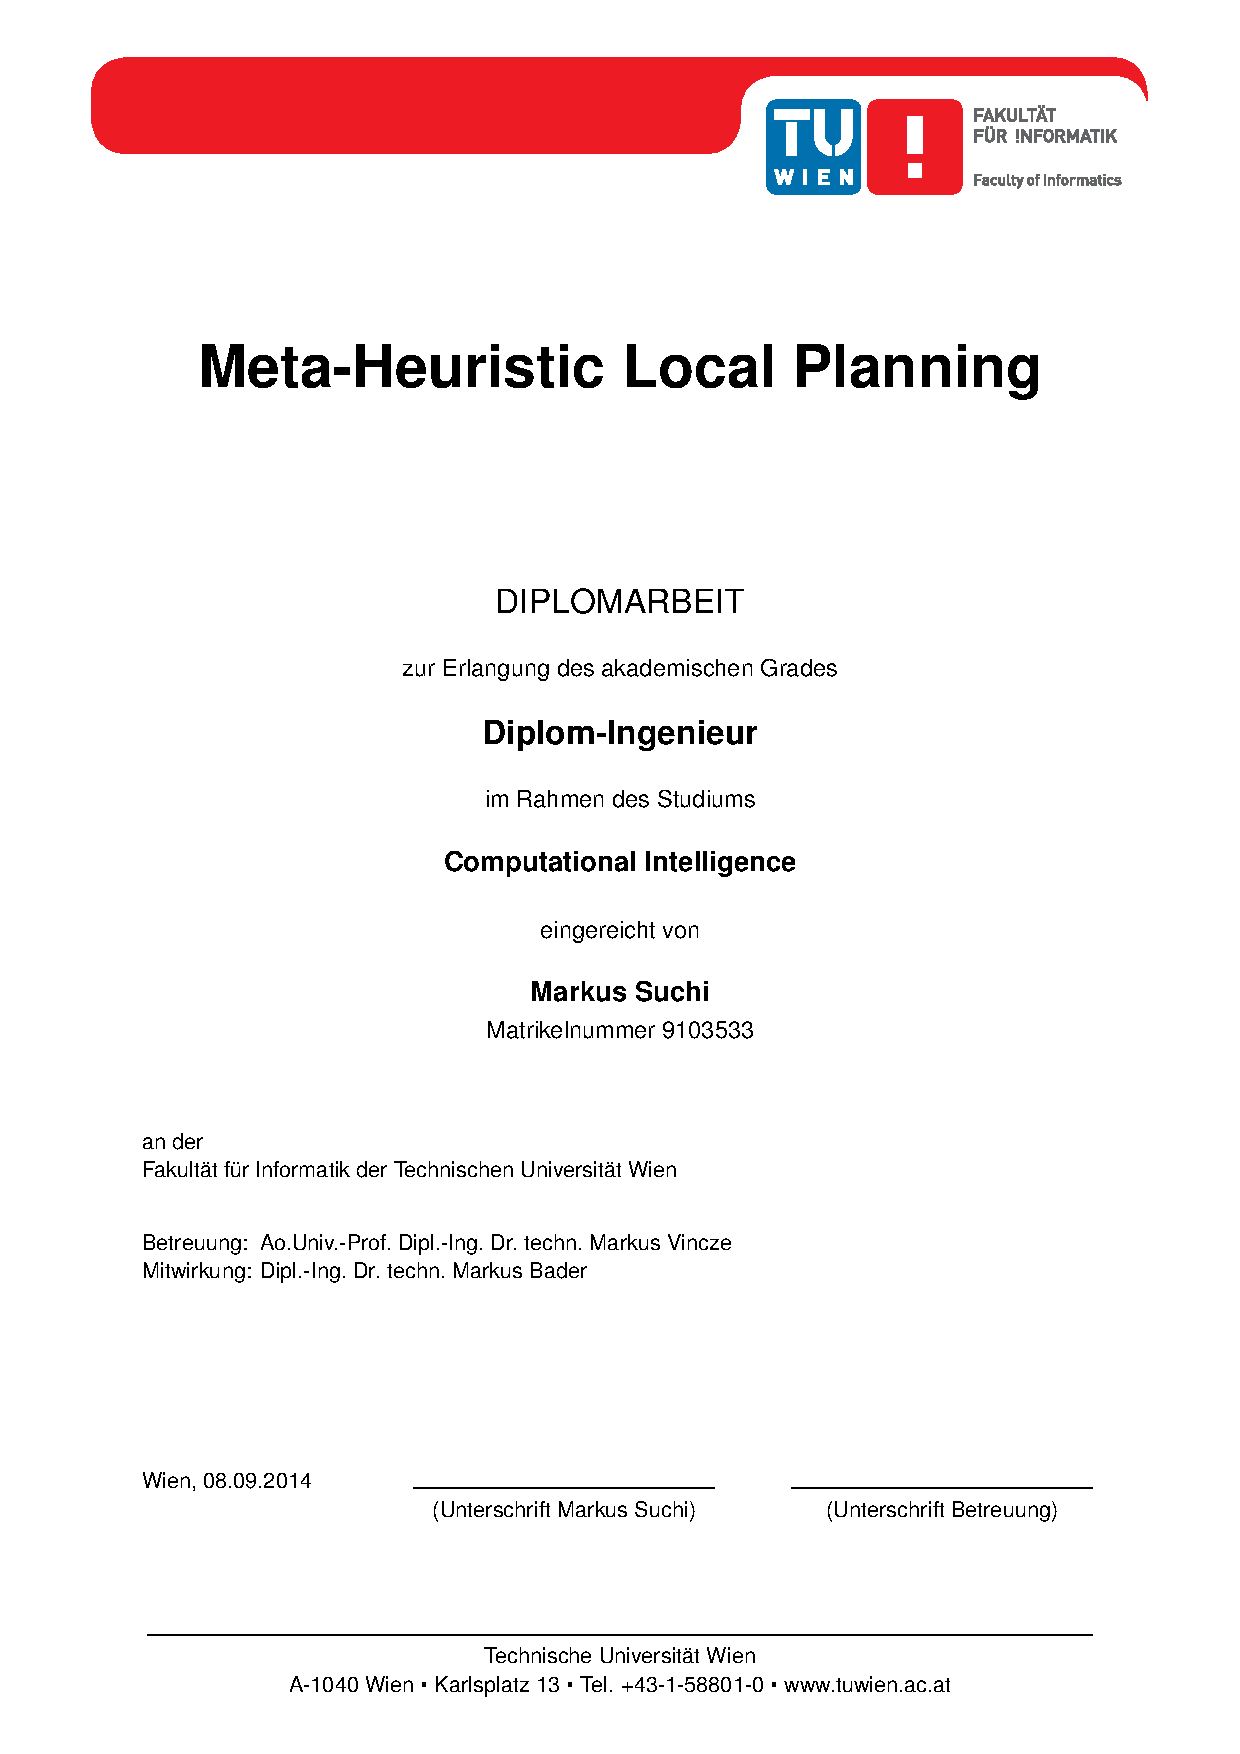
\includepdf[pages={1,2,3,4,5,6}]{frontpage}



\pagenumbering{roman}
\setcounter{page}{5}
\pagestyle{plain}
%********************************************************************
% Frontmatter
%*******************************************************
%%*******************************************************
% Little Dirty Titlepage
%*******************************************************
\thispagestyle{empty}
%\pdfbookmark[1]{Titel}{title}
%*******************************************************
\begin{center}
    \spacedlowsmallcaps{\myName} \\ \medskip                        

    \begingroup
        \color{Maroon}\spacedallcaps{\myTitle}
    \endgroup
\end{center}        

\cleardoublepage%*******************************************************
% Titlepage
%*******************************************************
\begin{titlepage}
	% if you want the titlepage to be centered, uncomment and fine-tune the line below (KOMA classes environment)
	\begin{addmargin}[-1cm]{-3cm}
    \begin{center}
        \large  

        \hfill

        \vfill

        \begingroup
            \color{Maroon}\spacedallcaps{\myTitle} \\ \bigskip
        \endgroup

        \spacedlowsmallcaps{\myName}

        \vfill

        
\includegraphics[width=6cm]{gfx/TFZsuperellipse_bw} \\ \medskip

        %\mySubtitle \\ \medskip   
        %\myDegree \\
        %\myDepartment \\                            
        %\myFaculty \\
        %\myUni \\ \bigskip

        \myTime\ -- \myVersion

        \vfill                      

    \end{center}  
  \end{addmargin}       
\end{titlepage}   
%\thispagestyle{empty}

\hfill

\vfill

\noindent\myName: \textit{\myTitle,} \mySubtitle, %\myDegree, 
\textcopyright\ \myTime

%\bigskip
%
%\noindent\spacedlowsmallcaps{Supervisors}: \\
%\myProf \\
%\myOtherProf \\ 
%\mySupervisor
%
%\medskip
%
%\noindent\spacedlowsmallcaps{Location}: \\
%\myLocation
%
%\medskip
%
%\noindent\spacedlowsmallcaps{Time Frame}: \\
%\myTime

%\cleardoublepage%*******************************************************
% Dedication
%*******************************************************
\thispagestyle{empty}
%\phantomsection 
\refstepcounter{dummy}
\pdfbookmark[1]{Dedication}{Dedication}

\vspace*{3cm}

\begin{center}
    \emph{Ohana} means family. \\
    Family means nobody gets left behind, or forgotten. \\ \medskip
    --- Lilo \& Stitch    
\end{center}

\medskip

\begin{center}
    Dedicated to the loving memory of Rudolf Miede. \\ \smallskip
    1939\,--\,2005
\end{center}
%\cleardoublepage\include{FrontBackmatter/Foreword}
%*******************************************************
% Abstract
%*******************************************************
%\renewcommand{\abstractname}{Abstract}
\pdfbookmark[1]{Abstract}{Abstract}
\begingroup
\let\clearpage\relax
\let\cleardoublepage\relax
\let\cleardoublepage\relax

\chapter*{Abstract}
Navigation is a crucial task for mobile robots driving through dynamic environments.
Besides the difficulties involved in finding a way from a starting to some goal location, the problem gets more difficult if unknown objects, dynamics of the robotic vehicle and uncertainties from sensor readings have to be taken into account.

To guarantee a safe passage common approaches divide the navigation task into two parts - global and local planning.
A global planner finds an initial path to the desired goal location based on a previous obtained map. The retrieved path is used as a guide for a local path planning component.
This local path planner uses so called local information obtained through recent sensor readings and applies obstacle avoidance strategies to safely and efficiently follow the guide as precise as possible. 

%Very effective local planning methods like the \ac{DWA} or Trajectory Roll-out are based on sampling the control space of the robot.
Very effective local planning methods like the Dynamic Window Approach (DWA) or Trajectory Roll-out are based on sampling the control space of the robot. 
For a short amount of time the application of these controls is simulated generating corresponding trajectories.
By using appropriate cost functions the resulting trajectories are weighted and the best one yields the optimal target values for the motor controller.

The goal of this thesis is to analyze these approaches and improve the performance of local planners by applying well known meta-heuristic search strategies in the trajectory selection process.

For this purpose an introduction to local planning and obstacle avoidance methods is presented, followed by discussing applicable single solution based meta-heuristics. 

%Approaches based on \ac{ILS}, \ac{VNS} and Tabu Search are implemented and tested using a sample planner based on \ac{DWA}.
Approaches based on Iterated Local Search (ILS), Variable Neighborhood Search (VNS) and Tabu Search are implemented and tested using a sample planner based on DWA. 
These algorithms are analyzed and evaluated using random created instances of sensor maps. Results are documenting a significant increase in performance compared to the brute force evaluation commonly used in local planner. 

%With the gained knowledge of these tests the \ac{VNS} approach is selected to substitute the selection process in a popular implementation of a local planner within \ac{ROS}.
With the gained knowledge of these tests the (VNS) approach is selected to substitute the selection process in a popular implementation of local planner within the Robot Operating System (ROS). 
%Two algorithms based on trajectory Roll-out (VNS-ROL) and \ac{DWA} (VNS-DWA) are developed and  evaluated using a sophisticated simulation engine.
Two algorithms based on trajectory Roll-out (VNS-ROL) and DWA (VNS-DWA) are developed and evaluated using a sophisticated simulation engine. 
The altered planner outperform the original implementations on all tested instances.
\vfill
\newpage

\pdfbookmark[1]{Zusammenfassung}{Zusammenfassung}
\chapter*{Zusammenfassung}
Navigation ist eine wesentliche Funktion f\"ur mobile Roboter, die sich in einer dynamisch ver\"anderbaren Umgebung bewegen. 
Neben der Schwierigkeit einen Weg von einem Startpunkt zu einem Zielpunkt zu finden, erh\"ohen sich die Anforderungen an die Planung sobald unbekannte Objekte, die Fahrdynamik des Roboters und Messunsicherheiten der Sensoren ber\"ucksichtigt werden m\"ussen. 

Um eine sichere Passage zu garantieren, wird die Navigation \"ublicherweise in zwei Schritte aufgeteilt - globale und lokale Planung. 
Ein globaler Planer findet anhand einer vorher erstellten Karte einen ersten Weg zum gew\"unschten Ziel. 
Der gefundene Weg fungiert dann als Orientierungshilfe f\"ur eine lokale Wegplanungskomponente. 
Der lokale Planer verwendet unter Ber\"ucksichtigung der aktuellsten Sensormessungen sogenannte lokale Informationen und Strategien zur Kollisionsvermeidung um sicher und effizient der Orientierungshilfe so exakt wie m\"oglich zu folgen. 

Sehr effektive lokale Planungsmethoden wie Dynamic Window Approach (DWA) oder Trajectory Roll-out basieren auf einem Sampling des Controlspace des Roboters. 
F\"ur einen kurzen Zeitraum wird die Applikation von Steuerwerten simuliert und die resultierenden Trajektorien generiert.  
Mithilfe geeigneter Kostenfunktionen werden die Trajektorien gewichtet und die Steuerwerte der besten Trajektorie werden and die Motorsteuerung weitergeleitet.

Das Ziel der vorliegenden Arbeit ist eine Analyse und eine Verbesserung der Leistung von lokalen Planern durch Einsatz bekannter metaheuristischer Suchstrategien bei der Selektion der Trajektorien.

Zu diesem Zweck wird eine Einf\"uhrung zu lokalen Planungsmethoden und Methoden der Kollisionsvermeidung pr\"asentiert, gefolgt von einer Diskussion zu \glqq single solution based\grqq  Metaheuristiken. 
Ans\"atze basierend auf Iterated Local Search (ILS), Variable Neighborhood Search (VNS) und Tabu Search werden implementiert und mit einem auf DWA basierenden einfachen Planer getestet. 
Diese Algorithmen werden anhand zuf\"allig erzeugter Sensorkarten analysiert und ausgewertet. 
Die Resultate dokumentieren eine signifikante Steigerung der Leistung verglichen mit der Brute-Force-Methode, die \"ublicherweise bei dieser Art lokaler Planung verwendet wird.

Mit dem durch diese Untersuchungen erworbenen Wissen wird der VNS Ansatz gew\"ahlt um den Selektionsprozess in einer existierenden Implementierung von lokalen Planern innerhalb des Robot Operating Systems (ROS) zu ersetzen. 
Zwei Algorithmen basierend auf Trajectory roll-out (VNS-ROL) und DWA (VNS-DWA) werden entwickelt und mit einer modernen Simulationssoftware evaluiert. 
Die Leistung der adaptierten Planer \"ubertrifft dabei die \"ursprünglichen Implementierungen in allen getesteten Szenarien. 

\endgroup			

\vfill
%\cleardoublepage%*******************************************************
% Publications
%*******************************************************
\pdfbookmark[1]{Publications}{publications}
\chapter*{Publications}
Some ideas and figures have appeared previously in the following publications:

\bigskip

\noindent Put your publications from the thesis here. The packages \texttt{multibib} or \texttt{bibtopic} etc. can be used to handle multiple different bibliographies in your document.
%\cleardoublepage%*******************************************************
% Acknowledgments
%*******************************************************
\pdfbookmark[1]{Acknowledgments}{acknowledgments}

\begin{flushright}{\slshape    
    We have seen that computer programming is an art, \\ 
    because it applies accumulated knowledge to the world, \\ 
    because it requires skill and ingenuity, and especially \\
    because it produces objects of beauty.} \\ \medskip
    --- \defcitealias{knuth:1974}{Donald E. Knuth}\citetalias{knuth:1974} \citep{knuth:1974}
\end{flushright}



\bigskip

\begingroup
\let\clearpage\relax
\let\cleardoublepage\relax
\let\cleardoublepage\relax
\chapter*{Acknowledgments}
Put your acknowledgments here.

Many thanks to everybody who already sent me a postcard!

Regarding the typography and other help, many thanks go to Marco 
Kuhlmann, Philipp Lehman, Lothar Schlesier, Jim Young, Lorenzo 
Pantieri and Enrico Gregorio\footnote{Members of GuIT (Gruppo 
Italiano Utilizzatori di \TeX\ e \LaTeX )}, J\"org Sommer, 
Joachim K\"ostler, Daniel Gottschlag, Denis Aydin, Paride 
Legovini, Steffen Prochnow, Nicolas Repp, Hinrich Harms, 
 Roland Winkler, J\"org Weber, 
 and the whole \LaTeX-community for support, ideas and 
 some great software.

\bigskip

\noindent\emph{Regarding \mLyX}: The \mLyX\ port was intially done by 
\emph{Nicholas Mariette} in March 2009 and continued by 
\emph{Ivo Pletikosi\'c} in 2011. Thank you very much for your 
work and the contributions to the original style.


\endgroup




\pagestyle{scrheadings}
\cleardoublepage%*******************************************************
% Table of Contents
%*******************************************************
%\phantomsection
\refstepcounter{dummy}
\pdfbookmark[1]{\contentsname}{tableofcontents}
\setcounter{tocdepth}{2} % <-- 2 includes up to subsections in the ToC
\setcounter{secnumdepth}{3} % <-- 3 numbers up to subsubsections
\manualmark
\markboth{\spacedlowsmallcaps{\contentsname}}{\spacedlowsmallcaps{\contentsname}}
\tableofcontents 
\automark[section]{chapter}
\renewcommand{\chaptermark}[1]{\markboth{\spacedlowsmallcaps{#1}}{\spacedlowsmallcaps{#1}}}
\renewcommand{\sectionmark}[1]{\markright{\thesection\enspace\spacedlowsmallcaps{#1}}}
%*******************************************************
% List of Figures and of the Tables
%*******************************************************
\clearpage

\begingroup 
    \let\clearpage\relax
    \let\cleardoublepage\relax
    \let\cleardoublepage\relax
    %*******************************************************
    % List of Figures
    %*******************************************************    
    %\phantomsection 
    \refstepcounter{dummy}
    %\addcontentsline{toc}{chapter}{\listfigurename}
    \pdfbookmark[1]{\listfigurename}{lof}
    \listoffigures

    \vspace*{8ex}
    
    %*******************************************************
    % List of Algorithms
    %*******************************************************
    %\phantomsection 
    \refstepcounter{dummy}
    %\addcontentsline{toc}{chapter}{\listtablename}
    \renewcommand{\listalgorithmname}{List of Algorithms}  
         \addtocontents{loa}{\def\string\figurename{Algorithm}}
    \pdfbookmark[1]{List of Algorithms}{loa}
     \listofalgorithms
     \addtocontents{loa}{\def\string\figurename{Algorithm}}
        
    \vspace*{8ex} 

    %*******************************************************
    % List of Tables
    %*******************************************************
    %\phantomsection 
    \refstepcounter{dummy}
    %\addcontentsline{toc}{chapter}{\listtablename}
    \pdfbookmark[1]{\listtablename}{lot}
    \listoftables
        
    \vspace*{8ex}
%   \newpage

    %*******************************************************
    % List of Listings
    %*******************************************************      
	  %\phantomsection 
    %\refstepcounter{dummy}
    %\addcontentsline{toc}{chapter}{\lstlistlistingname}
    %\pdfbookmark[1]{\lstlistlistingname}{lol}
    %\lstlistoflistings 

    %\vspace*{8ex}
       
    %*******************************************************
    % Acronyms
    %*******************************************************
    %\phantomsection 
    \refstepcounter{dummy}
    \pdfbookmark[1]{Acronyms}{acronyms}
    \markboth{\spacedlowsmallcaps{Acronyms}}{\spacedlowsmallcaps{Acronyms}}
    \chapter*{Acronyms}
    \begin{acronym}[UML]
        \acro{DRY}{Don't Repeat Yourself}
        \acro{API}{Application Programming Interface}
        \acro{UML}{Unified Modeling Language}
    \end{acronym}                     
\endgroup

\cleardoublepage
%********************************************************************
% Mainmatter
%*******************************************************
\pagenumbering{arabic}
%\setcounter{page}{90}
% use \cleardoublepage here to avoid problems with pdfbookmark
\cleardoublepage
\part{Introduction}
%************************************************
\chapter{Introduction}\label{ch:introduction}
%************************************************
Navigation and planning are essential for mobile robots to act in out- and indoor environments. 
From self driving cars navigating 132~miles through the Mojave desert, or mobile robots handling goods in distribution centers and warehouses to mobile robots used for planetary exploration, autonomous robots have conquered nearly every place on earth and beyond.
 
Articles like \cite{stanley} and \cite{kiva} present the relationship between the environmental complexity and the computational on-board processing power needed to tackle the navigation problem.
The self driving car Stanley has a six processor computing platform provided by Intel whilst Kiva robots are using low cost DSP's for navigation and vision processing\footnote{Kiva Systems Uses "Smart" Blackfin-powered Robots for Warehouse Navigation | Analog Devices: \url{http://www.analog.com/en/content/kiva_systems_bf548/fca.html}} to drive within a known environment.  

While the application domains and computational powers varies strongly between the robotic systems, all of them have to move safely and efficient from one location to another.   

In this thesis we propose a method for improving navigation for mobile robots by the use of combining local planning methods with search strategies based on meta-heuristics.

This enables the local planner to:
\begin{itemize}
\item run at a higher frequency
\item simulate trajectories for a longer time interval
\item moving the robot at higher speed
\item investigate a larger amount of trajectories
\item use a higher costmap resolution
\end{itemize}

In order to give an impression of the importance of navigation and planning in the field of mobile robotics the next section gives some motivation and application examples.

\section{Motivation and Applications}\label{sec:motivation} 
The goal of navigation encompasses the ability of robots to find a series of actions based on its knowledge of the environment and sensor values to reach its goal position in an effective and efficient manner.
The resulting series of actions is called a \emph{plan}. 

To ensure safety and flexibility in the presence of obstacles in a dynamic environment \emph{obstacle avoidance} is used to alter plans during execution and generating of collision free trajectories.

A common strategy to deal with complex navigation problems is to the divide the planning task into a global and a local planning problem \cite{LaValle2006}.

Global path-planning usually operates on a simplified representation of the environment and the robot itself (e.g. static map, circle representation of the robots outline) to efficiently compute an optimal shortest path using variants of Dijkstra's \cite{dijkstra1959note} or $A^*$ \cite{DBLP:journals/tssc/HartNR68/Astar} algorithm, ignoring kinematic and acceleration constraints of the robot.
In succession the retrieved global path is used by a local planner for guiding the robot through the environment.
Figure~\ref{fig:fig_pioneer} illustrates the view of the environment from a robot perspective together with a global and local plan, which enables the robot to drive autonomous within our lab/office environment.

\begin{figure}[thpb]
      \centering
      \def\svgwidth{\textwidth}
      \includesvg{figures/pioneer_costmap}
      \caption[Global and local planning.]{This figure shows a Pionner3DX and its view of the office environment while passing through a door. The blue line shows the global path and the green line the selected trajectory of the local planner.}
      \label{fig:fig_pioneer}
\end{figure}

The major responsibility for local planner is obstacle avoidance. It takes sensor readings of the robot into account and is reactive to changes within the sensor range. 
It selects the best values of available motor controls in respect to the kinematic and dynamic constraints of the robot, generating collision free trajectories. 
   
Navigation competence is essential for a broad spectrum of application domains within the field of mobile robotics which are presented below:

\begin{description}
\item[Self driving cars]\hfill \\
Self driving cars (see Figure~\ref{fig:fig_auto}) like Stanley \cite{stanley} which won the 2005 DARPA (Defense Advanced Research Projects Agency of the United States) Grand Challenge and the Google car \cite{guizzo2011google} are two examples which illustrate the enormous potential of autonomous vehicles.
While the former is confronted with rough terrain and manoeuvrs at high speeds, cars in urban traffic have to be prepared for other vehicles, pedestrians and have to incorporate traffic rules into the navigation task. 

\begin{figure}[thpb]
	  \myfloatalign
      \footnotesize
      \centering
    \subfloat[Stanley (taken from \cite{stanley}).]
    {  \label{fig:fig_stanley}
        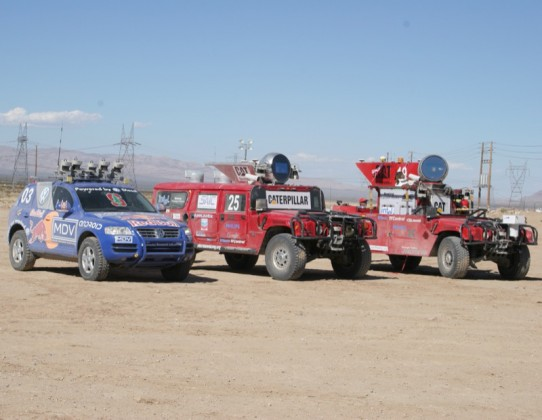
\includegraphics[width=0.55\textwidth,height=0.2\textheight]{figures/fig_stanley.jpg}
    }    
    \subfloat[Google car (Credit: Google\protect\footnotemark).]
    {  \label{fig:fig_googlecar}
       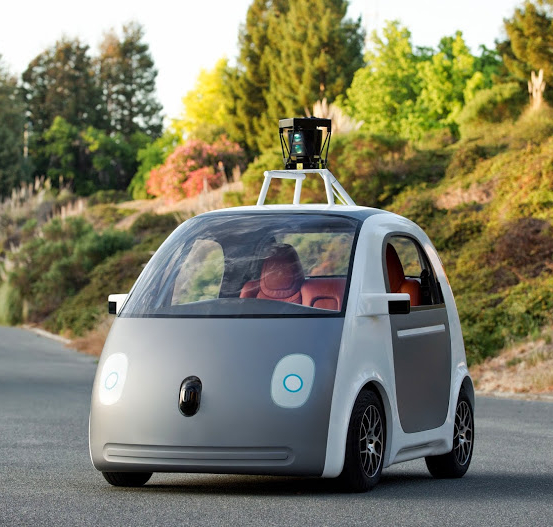
\includegraphics[width=0.45\textwidth,height=0.2\textheight]{figures/fig_googlecar.jpg}
    }
   \caption[Selfdriving car]{Self driving cars designed for different environments. On the left the winner of the 2005 DARPA Grand Challenge tackled wreckless driving through the Mojave desert and the right picture shows the new Google car designed for urban traffic.}
   \label{fig:fig_auto}
\end{figure}

\item[Planetary exploration]\hfill \\
Another example of autonomous vehicles are planetary rovers.
Three generations of Mars rovers developed at NASA are shown in Figure~\ref{fig:fig_nasa}. 
The first Mars rover, Sojourner, which landed on Mars in 1997 as part of the Mars Pathfinder Project was remotely operated from earth. 
The next generation of rovers, Spirit and Opportunity which landed 2004, did already have an autonomous navigation system. This enabled the robots to avoid hazardous situations without human intervention. 
The latest rover Curiosity is on its mission on Mars since August 2012 using autonomous navigation to explore mars on safe paths without the need of being remotely controlled by human operators.

An overview of recent developments in the field of planetary exploration including navigation topics can be found in \cite{PavoneAcikmese2014rover}.

\begin{figure}[thpb]
	  \myfloatalign
      \footnotesize
      \centering
    \subfloat[NASA Mars rover (Credit: NASA JPL-Caltech).]
    {  \label{fig:fig_nasa}
        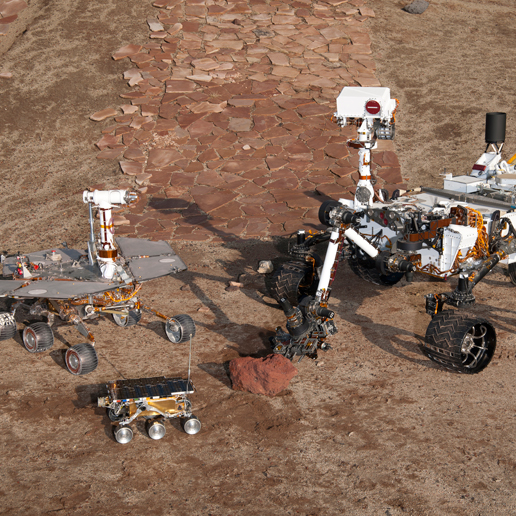
\includegraphics[width=0.45\textwidth,height=0.2\textheight]{figures/fig_marsrover.jpg}
        %\caption{Dijkstra}
    }
    \subfloat[Mawson rover (taken from \cite{Allister2012rover}).]
    {  \label{fig:fig_rover}
        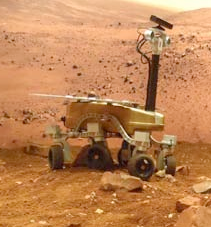
\includegraphics[width=0.45\textwidth,height=0.2\textheight]{figures/fig_rover.png}
        %\caption{Dijkstra}
    }     
   \caption[Mars rover]{Different Mars rover for planetary exploration. On the left Sojourner, Spirit and Curiosity from NASA which provided rich scientific information exploring Mars and on the right Mawson an academic research project on a training track at the Museum of Sydney.}
   \label{fig:fig_rovers}
\end{figure}
\footnotetext{Google self driving car available from \url{http://googleblog.blogspot.co.at/2014/05/just-press-go-designing-self-driving.html}}

\item[Search and Rescue]\hfill \\
Mobile robots provide a useful tool for rescue teams, whenever human intervention is not possible due to imminent risk of health and life, like immediate explosion hazard or threat of nuclear radiation.  
Figure~\ref{fig:fig_rescue} shows two prominent representatives of search and rescue robots.
\begin{figure}[thpb]
	  \myfloatalign
      \footnotesize
      \centering
    \subfloat[Pioneer (Credit: Carnegie Mellon University)]
    {  \label{fig:fig_chernobyl}
        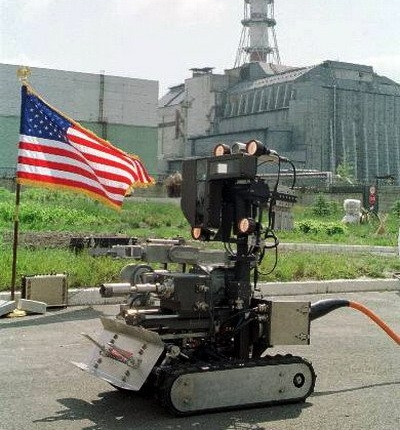
\includegraphics[width=0.45\textwidth,height=0.2\textheight]{figures/fig_chernobyl_pioneer.jpg}
        %\caption{Dijkstra}
    }
    \subfloat[Packbot (Credit: iRobot)]
    {  \label{fig:fig_fukushima}
        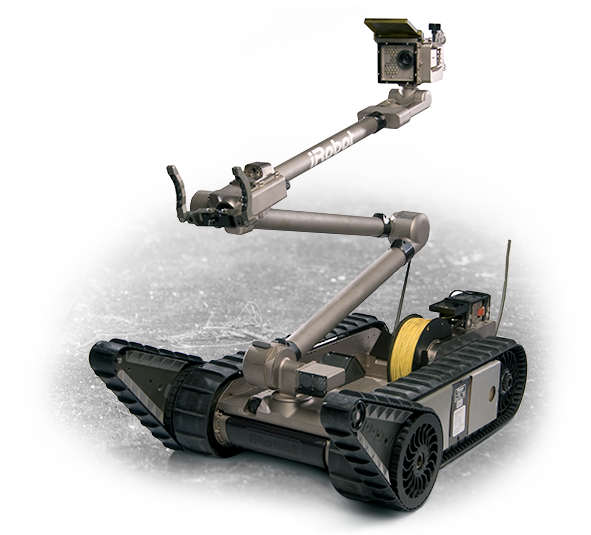
\includegraphics[width=0.45\textwidth,height=0.2\textheight]{figures/fig_packbot.png}
        %\caption{Dijkstra}
    }     
   \caption[Rescue robots]{Search and rescue robots are useful tools for human rescue teams. The left figure shows Pioneer at the nuclear disaster site in Chernobyl, the right robot shows a Packbot which operated in the nuclear power plant in Fukushima.}
   \label{fig:fig_rescue}
\end{figure}

The robot PIONEER sponsored by the US Department of Energy and NASA was the first of its kind to be deployed to the remnants of the nuclear power station in Chernobyl in the Ukraine after the supergau in 1986. 
The robots mission was to evaluate the sarcophagus which was built to shield off radiation.

In 2011 after an earthquake caused a nuclear disaster at the Fukushima Daiichi power plant in Japan, two PACKBOT robots of the American company iRobot were deployed to perform on site observations.

While the aforementioned robots were remotely operated, autonomous robots are a hot research topic in the academic domain. In the last 5 years more than 90 teams from universities participated in RoboCup competitions and already provide impressive results like Hector \cite{2014:hector_rescue_tdp} the winner of the 2014 RoboCup Rescue League world championship.

\item[Assistance]\hfill \\
Besides robots acting in outdoor environments, assistance robots have to cope with the difficulties involved in operating side by side with humans in indoor environments. 
Obstacles like desks and chairs located in small corridors and rooms pose a challenging navigation problem.
Tour guide robots like Rhino \cite{DWA1997} and Robox \cite{philippsen:2004:phd} are especially designed to deal with this kind of setting.
Figure~\ref{fig:fig_robox} shows Robox at the Robotics@Expo.02 event. 

Figure~\ref{fig:fig_hobbit} shows the robot Hobbit \cite{fischinger2013hobbit}\cite{zagler2014roboter} which goes one step further in assisting elderly people in their everyday activities.
It does not only make an excellent job in dealing with the pitfalls of navigating in indoor environments, in addition it is equipped with the capabilities to identify and to remove obstacles on the floor to provide safe passages for its human users.

\begin{figure}[thpb]
	  \myfloatalign
      \footnotesize
      \centering
    \subfloat[Hobbit (taken from \cite{fischinger2013hobbit})]
    {  \label{fig:fig_hobbit}
        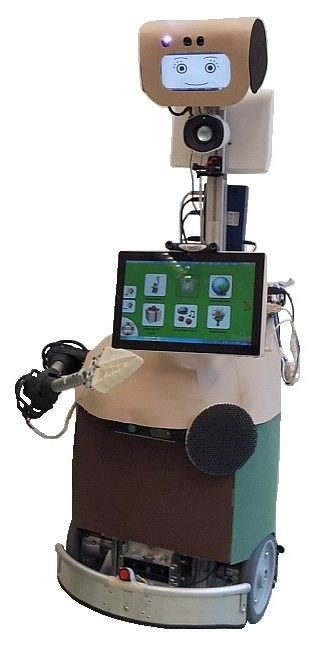
\includegraphics[width=0.40\textwidth,height=0.34\textheight]{figures/fig_hobbit.png}
        %\caption{Dijkstra}
    }
    \subfloat[Robox (taken from \cite{philippsen:2004:phd})]
    {  \label{fig:fig_robox}
        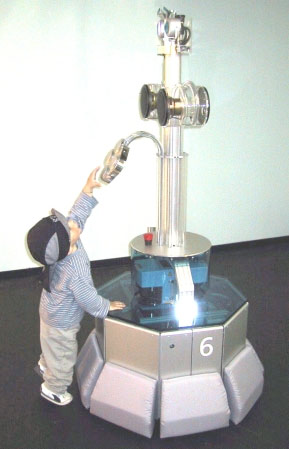
\includegraphics[width=0.40\textwidth,height=0.34\textheight]{figures/fig_robox.png}
        %\caption{Dijkstra}
    }     
   \caption[Assitance robots]{Hobbit the \emph{care} robot supporting elderly people and Robox working as a tour guide.}
   \label{fig:fig_assist}
\end{figure}

\item[Logistics and Transportation]\hfill \\
Automated guided vehicles (AGV) are an essential part in industry to support automated manufacturing. Figure~\ref{fig:fig_agv} shows a typical AGV from the Austrian company DS-Automotion.
The mobile robots follow markers, wires, or magnets in the floor, and make use of lasers and computer vision methods to accomplish navigation tasks. 
Their main responsibility is to move materials safely and efficient around manufacturing facilities, warehouses (eg. Kiva Systems \cite{kiva}) or hospitals (eg. HELPMATE \cite{ROB:4520696}). 

If transportation by road is not possible a flying drone might do the job. Projects from major companies like Googles \emph{project wing}\footnotetext{Project Wing delivery drones \url{https://plus.google.com/+google/posts/TqrsvRyPeNH}} and Amazons \emph{Prime Air} are working on self flying drones to deliver packages. 
Figure~\ref{fig:fig_uav} shows a prototype drone on a test flight. 

\begin{figure}[thpb]
	  \myfloatalign
      \footnotesize
      \centering
    \subfloat[AGV (Credit: DS-Automotion)]
    {  \label{fig:fig_agv}
        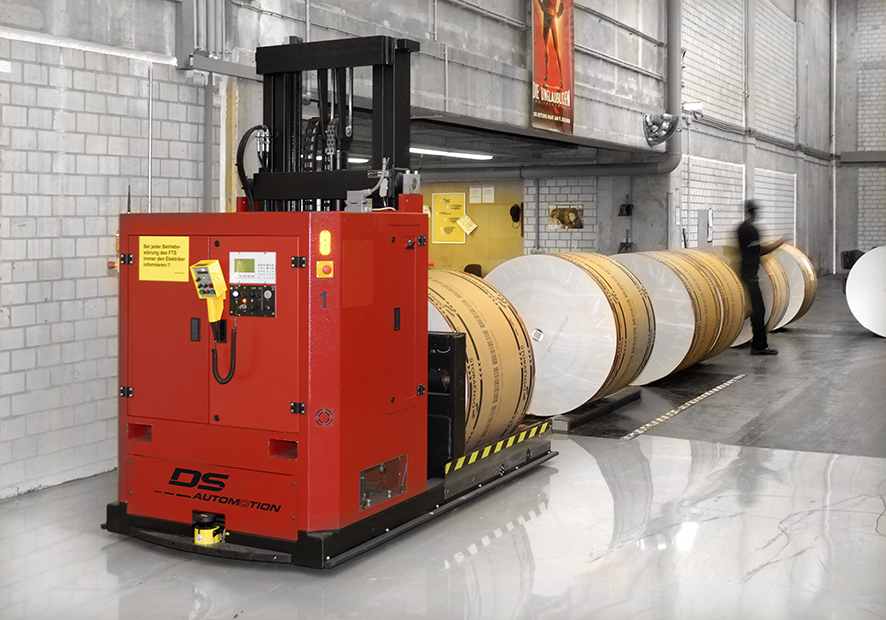
\includegraphics[width=0.45\textwidth,height=0.2\textheight]{figures/fig_AGV-dsautomation.jpg}
        %\caption{Dijkstra}
    }
    \subfloat[Project Wing delivery drone (Credit: KEYSTONE)]
    {  \label{fig:fig_uav}
        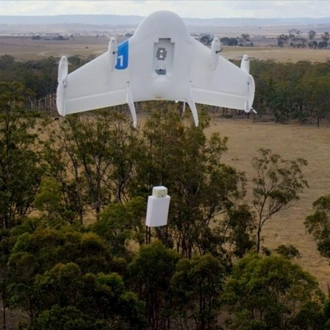
\includegraphics[width=0.45\textwidth,height=0.2\textheight]{figures/fig_wing.jpg}
        %\caption{Dijkstra}
    }     
   \caption[Logistic robots]{Transportation on earth using Automated Guided Vehicles and in the air with the support of self flying drones.}
   \label{fig:fig_transport}
\end{figure}

\item[Commercial]\hfill \\
Robots play a vital role in the manufacturing of goods. Besides classical domains such as  automotive industry, robots are used for mining, construction and maintenance tasks. 
For example DeWaLoP, shown in figure~\ref{fig:inpipe}, is used for cleaning fresh water pipes, navigating through a 3000 km pipeline network in Vienna \cite{mateos2013inpipe}.   

The employment of autonomous robots is also a field of attention in agriculture. 
Monitoring, harvesting and precision spraying pesticides of crops have to be carefully accomplished without hurting fragile plants. 
Figure \ref{fig:fig_cropbot} shows a harvesting robot developed at the Technische Universit\"at M\"unchen moving in a greenhouse \cite{Schuetz2014}.

\begin{figure}[thpb]
	  \myfloatalign
      \footnotesize
      \centering
    \subfloat[DeWaLoP (taken from \cite{mateos2013inpipe})]
    {  \label{fig:inpipe}
        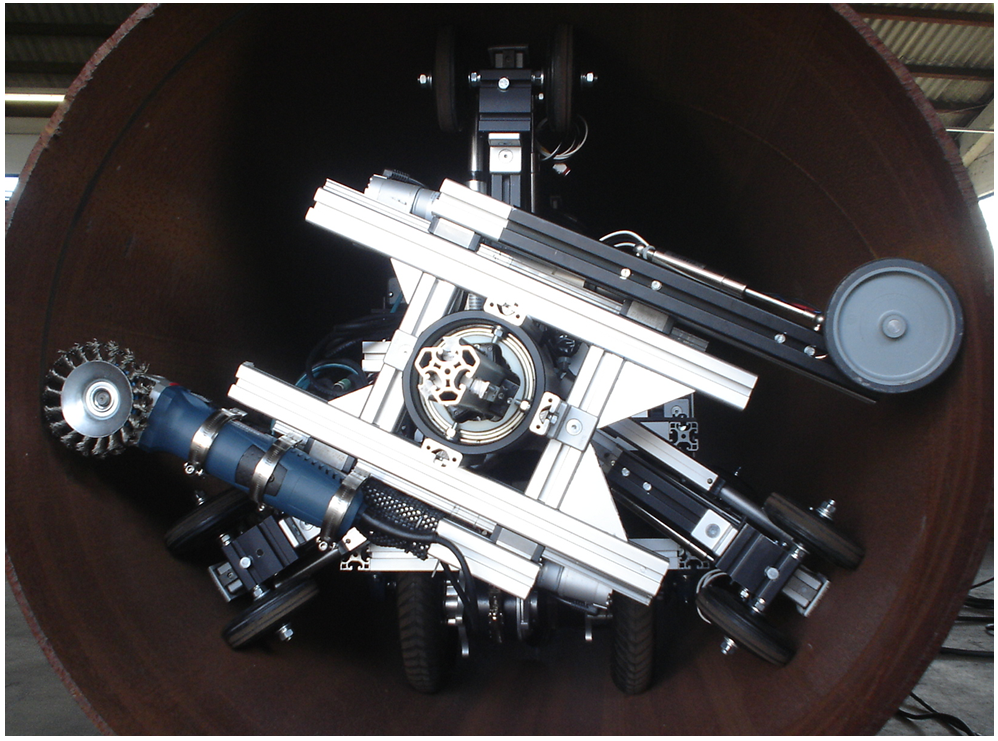
\includegraphics[width=0.45\textwidth,height=0.2\textheight]{figures/fig_inpiperobot.png}
        %\caption{Dijkstra}
    }
    \subfloat[Harvesting robot (taken from \cite{Schuetz2014})]
    {  \label{fig:fig_cropbot}
        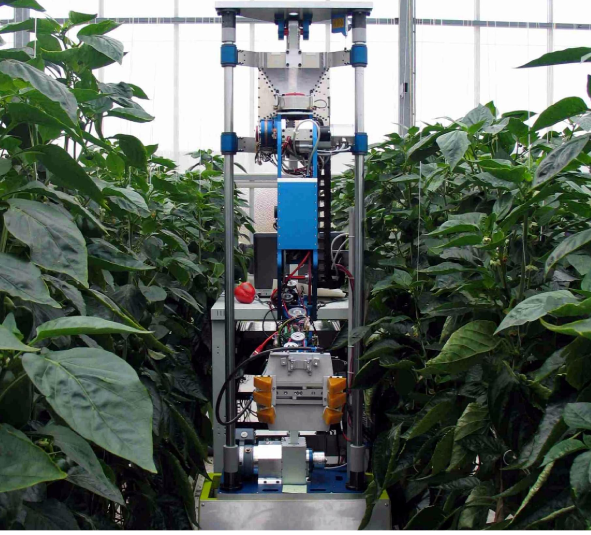
\includegraphics[width=0.45\textwidth,height=0.2\textheight]{figures/fig_croprobot.png}
        %\caption{Dijkstra}
    }     
   \caption[Commercial robots]{The right figure shows an in-pipe maintenance robot, the left image an agricultural robot used for harvesting and spraying of sweet-pepper crops.}
   \label{fig:fig_commercial}
\end{figure}

\item[Challenges and Competitions]\hfill \\
Attractive competitions have the purpose to spur innovation and sponsor research development in the field of robotics .  
One of the most popular events are organized and sponsored by DARPA. Besides the already mentioned Grand Challenge for wreckless self driving cars, the successor events DARPA Urban Challenge focused on autonomous vehicles moving in urban areas. 
In 2012 the first DARPA Robotics Challenge took place which provided a platform for wheeled and humanoid search and rescue robots.

World Competitions of soccer playing robots fascinate and motivate thousands of people every year and have a significant impact on the development of innovative methods including navigation and planning for mobile robots.
Figure~\ref{fig:fig_competition} shows wheeled and humanoid robots trying their best at scoring more goals than their opponents.
The biggest events are organized by FIRA\footnote{Federation of International Robot-soccer Association, founded in 1997. Details can be found at \url{www.fira.net}.} and RoboCup\footnote{RoboCup Federation, founded in 1993. Details can be found at \url{www.robocup.org}.}, which provide annual competitions for wheeled and humanoid soccer robots.

\begin{figure}[thpb]
	  \myfloatalign
      \footnotesize
      \centering
    \subfloat[MiroSot (taken from \url{www.fira.net})]
    {  \label{fig:mirosot}
        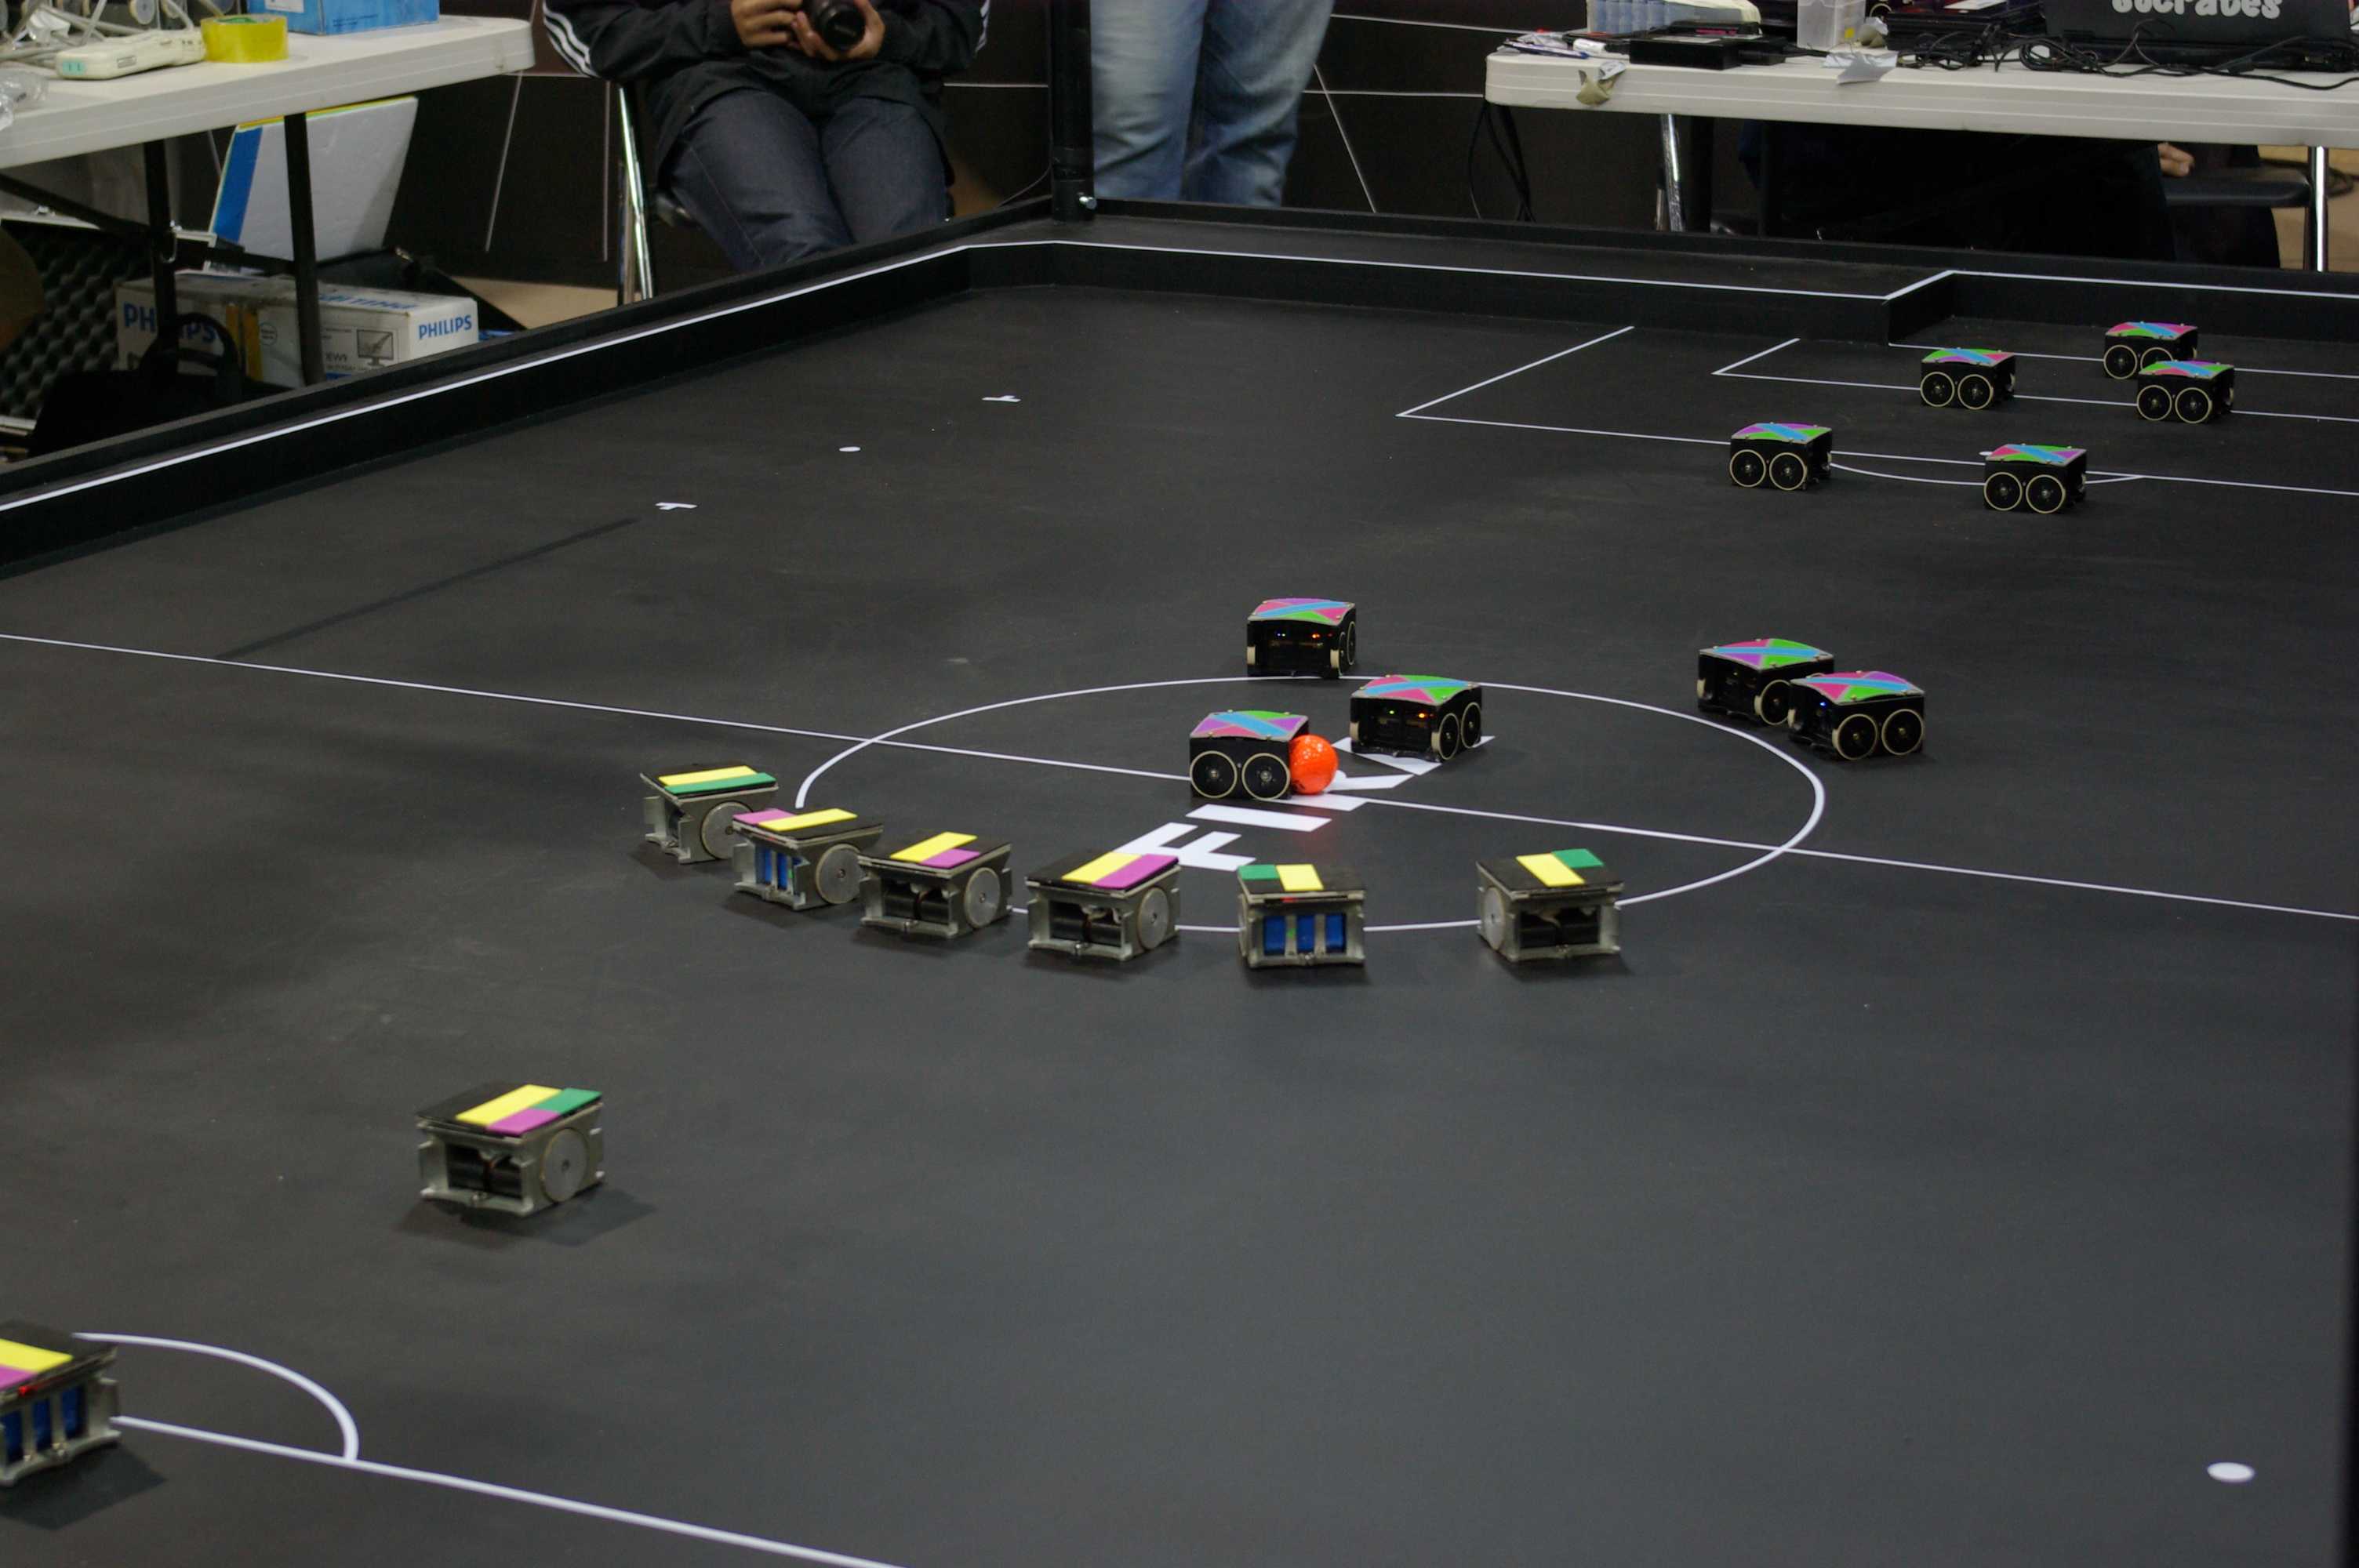
\includegraphics[width=0.45\textwidth,height=0.2\textheight]{figures/fig_mirosot.jpg}
        %\caption{Dijkstra}
    }
    \subfloat[Standard Platform League (taken from \url{www.robocup2014.org})]
    {  \label{fig:fig_naosoccer}
        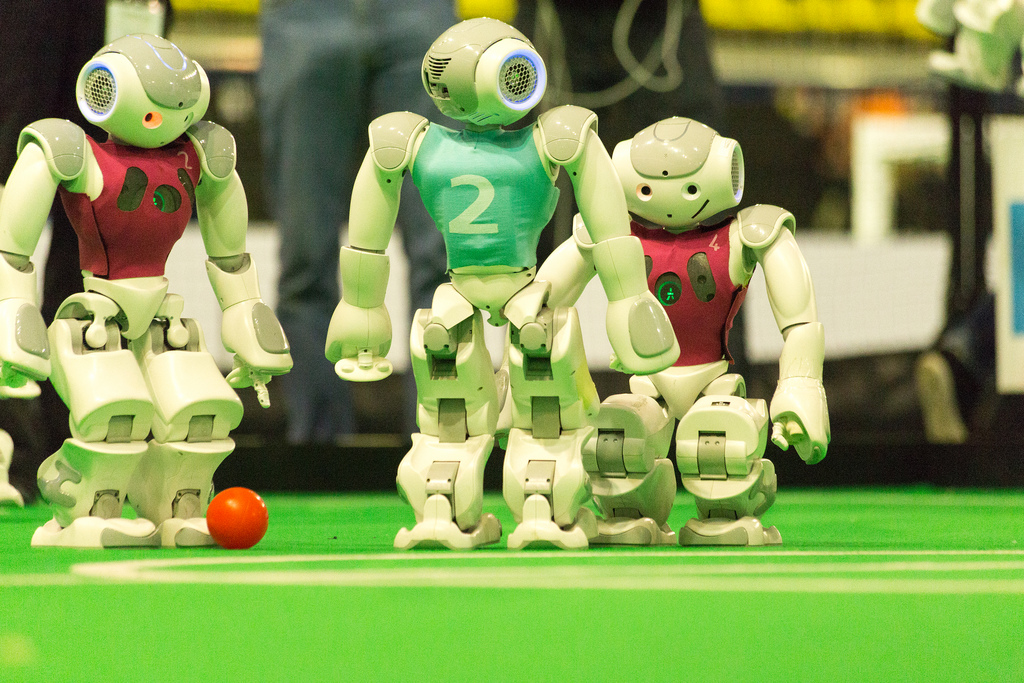
\includegraphics[width=0.45\textwidth,height=0.2\textheight]{figures/fig_naosoccer.jpg}
        %\caption{Dijkstra}
    }     
   \caption[Soccer robots]{The right figure shows competitors of the MiroSot league, the left image humanoid Nao robots playing soccer in the RoboCup Standard Platform League.}
   \label{fig:fig_competition}
\end{figure}
\end{description}

All of these examples show that navigation plays an essential role in mobile robotics. Excellent planning algorithms are needed to enable a wide area of applications and allow autonomous and semi-autonomous machines to safely and economically move through in- and outdoor environments.

\section{Related Work}\label{sec:relwork}
Similar approaches using meta-heuristics are mostly present in the field of global planning. Especially population based meta-heuristic algorithms are used to tackle planning problems for single and multiple robots.

In \cite{zhou2010improvedantcolony} an ant colony optimization (ACO) algorithm is used to find global minimal paths for soccer robots. The algorithm uses a combination of cellular automata and a special designed pheromone model to find an initial global path. In a second step the retrieved path is smoothed and can be used to guide a robot.

In \cite{buniyamin2011robotantcolony} the performance of finding optimal shortest global paths by applying an ACO algorithm is documented. The proposed method uses a special heuristic to set the moving directions of the ants in the system based on shortest distance between nodes in the search graph.  



\section{Goal of Thesis and Scientific Contribution}\label{sec:goal}
The goal of this thesis is to provide an extension to local planning systems for mobile robots based on trajectory generation and parts of this work were presented at the Austrian Robotics Workshop 2014 \cite{myself}. 
The proposed method applies meta-heuristic search strategies to improve the performance of local planner based on brute force evaluation of a fixed number of trajectories.

This includes the following sub-goals.
\begin{description}
\item[Compilation of local planning approaches]\hfill \\
A detailed overview of local planning and obstacle avoidance methods has to be compiled. 
\item[Investigating possible meta heuristic algorithms]\hfill \\
Selection and adapting applicable meta-heuristics to make them usable for trajectory selection.
\item[Design of benchmark instances and sample planner]\hfill \\
Suitable test instances and a sample planning program which allow to set the focus of investigating the proposed method on the local planning task have to be developed.  
\item[Implementation]\hfill \\
The gained data from the benchmark instances and the sample planner are used to implement meta-heuristic local planning in an existing navigation system for mobile robots.  
\item[Evaluation]\hfill \\
Experiments have to be designed and evaluated to document the performance of the meta-heuristic algorithms in comparison to their unaltered counterparts.
\end{description}

\section{Outline}\label{sec:outline}
This work is structured in the following way. 
In Chapter \ref{ch:introductionplanning} the basic sources for planning are outlined, covering the basic problem definition, representation of the environment and different robotic motion models. 

Chapter \ref{ch:local} gives an overview of important local planning and obstacle avoidance methods.
 
Chapter \ref{ch:meta} represents the main part of this thesis and introduces meta-heuristic extensions to local planning methods. 
Starting with an detailed overview of  meta-heuristic algorithms, two application based on ILS and VNS are used for trajectory selection of a local planner and described in Section \ref{sec:trajselmeta}.

A detailed evaluation of these methods is presented in Chapter \ref{ch:eval}, using a very simple implementation of a local planner and randomly generated sensor maps. 
The gathered data is then used to implement a meta-heuristic trajectory selection in a high sophisticated planner and tested using simulation software with a robust physical engine.

Chapter \ref{ch:conc} concludes the work of this thesis with a short summary and an outlook on future research directions.
%*****************************************
%*****************************************
%*****************************************
%*****************************************
%*****************************************





%************************************************
\chapter{Basic Concepts}\label{ch:introductionplanning}
%************************************************
General Introduction to Thesis

\section{Classic Path Planning Problem}\label{sec:basic}
Statespace,
Workspace,
Configurationspace,
Obstacles in Configurationspace,
Actions,
Paths,
Trajectories,

\section{Representation of the Environment}\label{sec:representation}
Exact Cell Decomposition
Approximate Cell Decomposition
Visibility Graph
Voronoi Regions

\section{Robotic Models}\label{sec:model}
free, holonomic, nonholonimc
kinematics, dynamics
unicycle, differential drive, car-like 

\section{Planning}\label{sec:global}
Global Planning:
Breadth-First Search (BFS)
Depth-First Search (DFS)
Dijkstra's and A* algorithm
An illustration is given in Figure~\ref{fig:fig_overview}
\begin{figure}[thpb]
	  \myfloatalign
      \footnotesize
      \centering
    \subfloat[Dijkstra algorithm]
    {  \label{fig:fig_djikstra}
        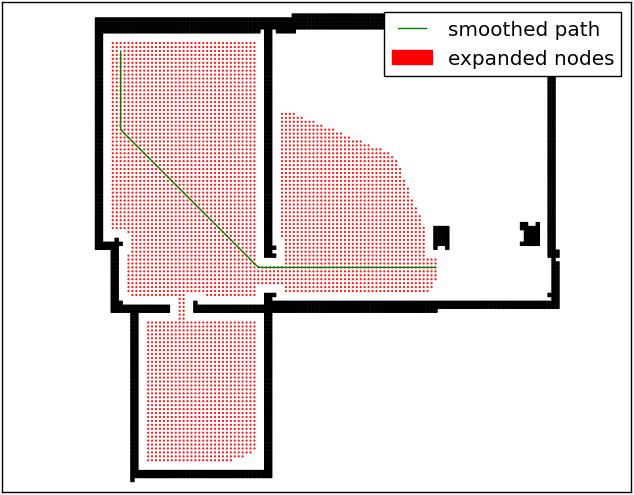
\includegraphics[width=0.75\textwidth]{figures/fig_djikstra.png}
        %\caption{Dijkstra}
    }
    
    \subfloat[A* algorithm]
    {  \label{fig:fig_astar}
       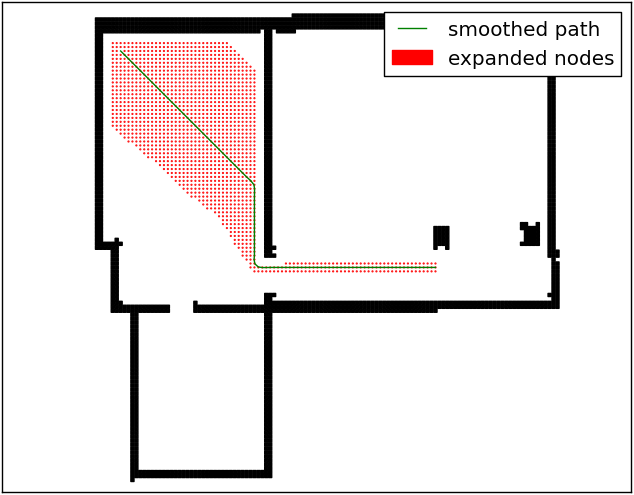
\includegraphics[width=0.75\textwidth]{figures/fig_astar.png}
       %\caption{A*}
    }
   \caption[Djikstra's and A* algorithm.]{The difference between Djikstra's and A* algorithm searching for a shortest path in a grid representation of a building. A* is more effective, as it visits by far less nodes in the search graph. }
\label{fig:fig_overview}
\end{figure}
Examples: 
Rapidly Exploring Randomized Trees (RRT)
Probabilistic Road Maps (PRM)
Potential Field

Local Planning:
The next chapter investigates local planning methods.

%*****************************************
%*****************************************
%*****************************************
%*****************************************
%*****************************************





%Chapter 03
%************************************************
\chapter{Planning Algorithms}\label{ch:planningalgorithms}
%************************************************
Overview and classification of path planning algorithms
\section{Global Planning}\label{sec:global}
\subsection{Graph Search}
\subsubsection{Breadth-First Search (BFS)}
\subsubsection{Depth-First Search (DFS)}
\subsubsection{Dijkstra's and A* algorithm}
An illustration is given in Figure~\ref{fig:fig_overview}
\begin{figure}[thpb]
	  \myfloatalign
      \footnotesize
      \centering
    \subfloat[Dijkstra algorithm]
    {  \label{fig:fig_djikstra}
        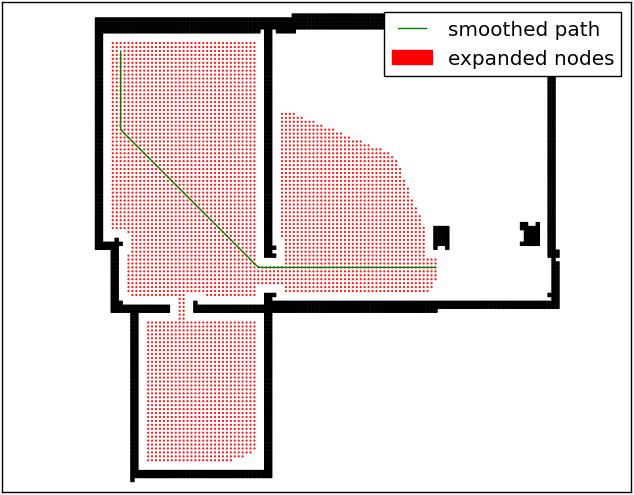
\includegraphics[width=0.75\textwidth]{figures/fig_djikstra.png}
        %\caption{Dijkstra}
    }
    
    \subfloat[A* algorithm]
    {  \label{fig:fig_astar}
       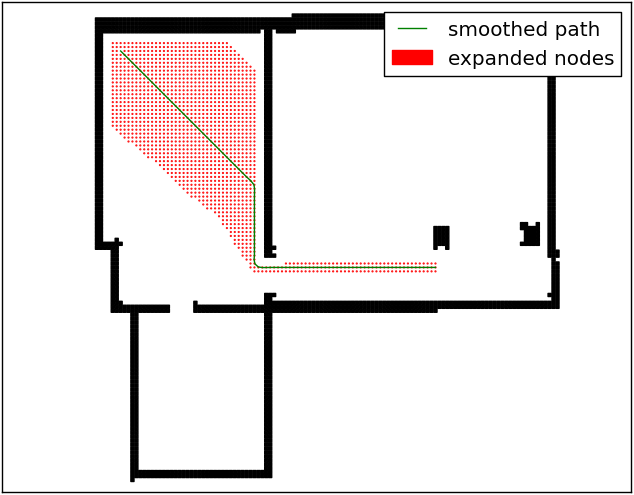
\includegraphics[width=0.75\textwidth]{figures/fig_astar.png}
       %\caption{A*}
    }
   \caption[Djikstra's and A* algorithm.]{The difference between Djikstra's and A* algorithm searching for a shortest path in a grid representation of a building. A* is more effective, as it visits by far less nodes in the search graph. }
   \label{fig:fig_overview}
\end{figure}
\subsection{Roadmap Based Navigation}
\subsubsection{Rapidly Exploring Randomized Trees (RRT)}
\subsubsection{Probabilistic Road Maps (PRM)}
\subsection{Potential Field}
\section{Local Planning and Obstacle Avoidance}\label{sec:local}
\subsection{Bug Algorithms}
\subsection{HistogramMehods}
M. I. Ribeiro. Obstacle avoidance. Institute for Systems and Robotics, [Online], Available:  \url{http://users.isr.ist.utl.pt/~mir/}, March 5, 2011.
Vector Field Histogram(VFH)
Nearness Diagrams (ND)
\subsection{Velocity Space Methods}
\subsection{Curvature Velocity Method (CVM)}
The Curvature Velocity Method in \cite{simmons1996curvature} is an obstacle avoidance method which considers kinematic and dynamic constraints of the robot and the environment.
These constraints are added to a \emph{velocity space} which consists of \emph{translational velocity} $v$ and \emph{rotational velocity} $w$.
One basic assumption of this approach is that the robot can only travel along circles with curvature $c=w/v$. 
This approximation neglects acceleration issues and restricts the robot motions to constant velocities over a given time horizon. 
  
Another simplification is the representation of obstacles as circles, which is used for fast transformation of the obstacles into the velocity space.
All curvatures which do not hit obstacles and adhere to the kinematic constraints of the robot are then evaluated using a cost function.
Since approximation techniques like simulated annealing to maximize the cost function using the whole velocity space did not succeed, the velocity space is divided into finite sets of curvature intervals.
The objective function is then evaluated over all curvature intervals.

\subsection{Dynamic Window Approach (DWA)}\label{sec:dwa}
A well known method for local planning is the Dynamic Window Approach proposed in \cite{DWA1997}. 
The method discretely samples the velocity space $(v,w)$ of the robot, where again $v$ is the \emph{linear velocity} and $w$ the \emph{angular velocity} of the robot, to create a set of feasible trajectories.
The velocity space is reduced to the reachable minimal and maximal velocity in one control cycle, taken the acceleration limits of the robot into account.
For a fixed amount of velocity samples the corresponding trajectories are created using a predefined granularity by performing forward simulation for a short period of time, starting at the current position of the robot. 
The trajectories which stop safely before an obstacles are called \emph{feasible}.
Evaluating all \emph{feasible} trajectories with respect to a weighted cost function (cf. Equation~\ref{eq:costfunction}) identifies the best velocity tuple, which is then forwarded to the motor controller.

\begin{equation}
   f_c(v,w)=\alpha f_a(v,w)+\beta f_d(v,w)+\gamma f_v(v,w)
   \label{eq:costfunction}
\end{equation}

The function $f_a(v,w)$ judges the angle between the robots heading and a given goal position.
It is maximal if the heading is a straight line to the goal.
The distance to the closest obstacle is calculated in the function $f_d(v,w)$.
The function $f_v(v,w)$ takes the forward velocity into account and rewards faster movements of the robot.
This method does not use a global plan to guide the robot, so without further changes it is subject to get captured in local minima.

Other applications of this approach in recent planning systems adapt the corresponding cost function. 
%give some recent papers about dwa in developments%
The excellent \texttt{move\_base}\footnote{move\_base planning framework: \url{http://wiki.ros.org/move_base}} motion planning framework introduced in \cite{DBLP:conf/icra/Marder-EppsteinBFGK10} implements within the navigation stack of Robot Operating System (ROS) a local planner which uses a global plan as a guide.

One implementation is based on DWA.
There is also the option to use Trajectory rollout \cite{gerkey08planning} as a local planner which is very related to the DWA, but in contrast improves in simulating the robots trajectory by accurately applying acceleration limits over the whole simulation time.
The cost function maximizes characteristics like proximity to obstacles, proximity to the goal, proximity to the global path, and speed.
Furthermore a number of escaping strategies try to avoid the vulnerability to local minima. 

Collision detection and cost calculation is performed by using the footprint of the robot following the calculated trajectory.
Hence the discretized footprint, which is usually given as a simple polygon, is projected on the costmap. 
Bresenham's Line algorithm \cite{bresenham1965algorithm} is used for ray-tracing the contour of a robot in the discrete workspace. 
Figure~\ref{fig:fig_global} shows the global view of the planning task. 
In Figure~\ref{fig:fig_local} the corresponding local view is depicted, including all sampled trajectories which are evaluated using a local costmap.

\begin{figure}[thpb]
	  \myfloatalign
      \footnotesize
      \centering
    \subfloat[Path planning in global costmap.]
    {  \label{fig:fig_global}
       \def\svgwidth{0.75\textwidth}
       \includesvg{figures/fig_global}

    } \\    
    \subfloat[Trajectory generation for linear, and angular velocities $(v,w)$ in local costmap guided by global path.]
    {  \label{fig:fig_local}
       \def\svgwidth{0.75\textwidth}
       \includesvg{figures/fig_local}
    }
   \caption[]{}
   \label{fig:fig_dwa}
\end{figure}

Concerning the optimization of the used cost functions the most common approach for DWA and related local planner is to evaluate all possible trajectories in a reduced discrete velocity space. 
Examples of this approach can be found in \cite{kiss2012advanced}\cite{DBLP:conf/icra/Marder-EppsteinBFGK10}\cite{conf/icra/SederP07}. 

The proposed method extends the DWA approach, by using approximation algorithm to maximize the cost function in a discrete representation of the velocity space.

%*****************************************
%*****************************************
%*****************************************
%*****************************************
%*****************************************





\cleardoublepage


\ctparttext{}


\part{Meta Heuristic Extended Local Planning}
% Chapter 4
\chapter{Meta Heuristic Extended Local Planning}\label{ch:meta}

In this chapter we propose an approach to extend local planning systems, which are based on trajectory simulation and evaluation. The main idea is to apply well established Meta-Heuristic search algorithms to find good trajectories within a given sample of different applicable velocities, a robotic motion model and a given time period for simulation. 

We introduce trajectory selection extensions using a combination of meta-heuristic algorithms.

\begin{itemize}
\item{\bf{RST:}}    Random Restart method using simple term memory
\item{\bf{ILS-Tabu:}}  Based on Iterated Local Search and the use of a simple memory
\item{\bf{VNSB-Tabu:}} Based on Variable Neighborhood Search and the use of a simple memory and Best Improvement heuristic.
\item{\bf{VNSF-Tabu:}} Based on Variable Neighborhood Search and the use of a simple memory and Best Improvement heuristic.
\end{itemize}

The proposed methods are tested and refined and implemented into a robotic navigation system which already supports implementations of a local planner based on Dynamic Window Approach and Trajectory Rollout.

\begin{itemize}
\item{\bf{VNSB-POSNEG}} Refining VNSB-Tabu with short term memory
\item{\bf{VNSF-POSNEG}} Refining VNSF-Tabu with short term memory
\end{itemize}

The next section provides background information of Meta-Heuristic search, followed by a detailed description about the specific algorithms used for extending local planners.

The relevant local planners we took into consideration are the aforementioned Dynamic Window Approach and Trajectory Roll-out planner, which will be discussed at the end of this chapter.

\section{Meta-Heuristic Search}
The family of Meta-Heuristics algorithms is extremely successful in solving optimization problems, and are heavily used to solve hard problems whether they are  \emph{discrete} (Combinatorial Problems: e.g. Traveling Salesman Problem (TSP), MAX-Sat problem, Nurse Rostering problems (NRP), Classical Vehicle Routing Problem (CVRP)), or \emph{real-valued} (Continuous Optimization Problems: e.g. Pooling problem, Continues Min-Max problem).

In general an optimization problem can be defined as follows (see \cite{blum2003metaheuristics}): 
\begin{definition}
An optimization problem $P = (S, f_c)$ can be defined by:\\
- a set of variables $X = \{x_1,\dots,x_n\} $;\\
- the values the variables can take (domains) $D_1,\dots,D_n$;\\
- constraints\\
- a cost function $f_c$ which has to be minimized, where $f_c:D_1 \times \dots \times D_n \rightarrow \mathbb{R}^+$; (which is the same as maximizing $-f_c$)\\
\end{definition}
The set of all possible assignments $S = \{s = \{(x_1,v_1),\dots,(x_n,v_n)\}\mid v_i \in D_i\}$ to the variables in $X$ is called the search or solution space.
A continues optimization problem is given if $S=\mathbb{R}^n$, otherwise if $S$ is discrete a discrete optimization problem is given.

Solutions which fulfill all constraints are called feasible solutions. 
It is not necessary to allow only feasible solutions in the search space, as accepting infeasible solutions during the search process can improve the overall solution quality and performance of the algorithm.

To solve an optimization problem one has to search the solution space to find a solution $s^*\in S$ with minimum costs. 
\begin{definition}
 A \emph{global} minimal solution is a solution $s^* \in S$ such that
 $f_c(s^*)\leq f_c(s) \forall s \in S$. 
\end{definition}
Since there might be more than one optimal solution $S^* \subseteq S$ is the set of \emph{globally} optimal solutions.

The main idea of meta-heuristic algorithms is to combine heuristic methods with strategic components which allow for an efficient and effective exploration of the search space. 

One basic heuristic approximation method is local search which given a initial solution tries to iteratively replace this solution with a better one in a defined neighborhood of the current solution. 
\begin{definition}
A neighborhood structure is a function $N:S\rightarrow 2^S$ that assigns to every $s \in S$ a set of neighbors $N(s) \subseteq S$. $N(s)$ is called the neighborhood of $s$.
\end{definition}
Defining the neighborhood function has an important influence on the good performance of many meta-heuristic algorithms. 
A neighborhood my be induced from metric functions introduced into $S$ given some notion of nearness within a given starting point. The process of a step from one local solution to another local solution is called a \emph{move}. Neighborhoods can also be induced by the set of applicable moves given a current solution (see \cite{gendreau2003tabusearch}).

Minimal solutions within a given neighborhood structure are defined as \emph{locally} minimal.
\begin{definition}
 A \emph{local} minimal solution w.r.t. a neighborhood structure $N$ is a solution $\hat{s}$  such that $\forall s_n \in N(\hat{s}):f_c(\hat{s})\leq f(s_n)$. 
\end{definition}
A visualization of the concepts of local vs. global minimal solutions is visualized in Figure~\ref{fig:fig_local_global}.
\begin{figure}[thpb]
   \footnotesize
   \centering
   \def\svgwidth{0.75\textwidth}
   \includesvg{figures/fig_local_global_minima}     
   \caption[]{This figures shows different kind of solutions to an optimization problem. The solutions $\hat{a}$ and $\hat{b}$ are local minimal solutions in the neighborhood $N_1(a)$ and $N_2(b)$ respectively, whereas the global minimal solution is $s^*$.}
   \label{fig:fig_local_global}
\end{figure}

\section{Single Solution Based Meta-Heuristics}
\subsection{Local Search}
The basic Local Search (LS) (cf. Algorithm~\ref{localsearchalgo}) finds a local optimum according to a cost function $cost(x)$ and a fixed sized region around an initial solution in the solution space. 
The set of solutions in this region is denoted as the neighborhood of $x$. The necessary steps to get from the initial solution to a solution in the neighborhood is called a move.

\begin{algorithm}
\caption{Local Search  (LS)}
\label{localsearchalgo}
\begin{algorithmic}[1] 
\State $x\gets$ initial solution
\Repeat
\State select a $x^\prime \in$ \Call{Neighborhood}{$x$}
\If {\Call{$cost$}{$x^\prime$} $\leq$ \Call{$cost$}{$x$}}
    \State $x\gets x^\prime$
\EndIf
\Until{stopping criteria satisfied}
\end{algorithmic}
\end{algorithm}

\subsection{Iterative Local Search}
A nice survey of Iterative Local Search including the basic algorithm (cf. Algorithm~\ref{ilsalgo}) can be found in \cite{lourencco2001iterated}. 
The main idea is to call a local search procedure iteratively, until a certain stopping criteria is satisfied. 
In each iteration the current solution might be perturbed by changing parts of the solution. 
The following local search takes this altered solution as a starting point and returns a new solution. 
If it satisfies an acceptance condition (e.g. the best solution so far), the process restarts with the new solution. 
In addition, a history of already found solutions may be used to steer perturbation and the acceptance test.
The steps of ILS are visualized in Figure~\ref{fig:fig_ils}

\begin{figure}[thb] 
   \footnotesize
   \centering
    \def\svgwidth{0.75\textwidth}
    \includesvg{figures/fig_ils}
    \caption[Pertubation step in ILS]{Pertubation of a local minimal solution $\hat{s}$, leads to an intermediate solution $s^\prime$. A local search is applied and a new local minimal solution $\hat{s}^\prime$ is found. (reproduced from \cite{blum2003metaheuristics})}  
     \label{fig:fig_ils}
\end{figure}
 
\begin{algorithm}
\caption{Iterative Local Search (ILS)}
\label{ilsalgo}
\begin{algorithmic}[1]
\State $x_0\gets$ initial solution
\State $x^*\gets$ \Call{LocalSearch}{$x_0$}
\Repeat
\State $x^\prime \gets$ \Call{Perturbation}{$x^{*}$,history}
\State $x^{*\prime} \gets$ \Call{LocalSearch}{$x^\prime$}
\State $x^* \gets$ \Call{AcceptanceCriterion}{$x^{*}$,$x^{*\prime}$,history}
\Until{stopping criteria satisfied}
\end{algorithmic}
\end{algorithm}

\subsection{Variable Neighborhood Search}
Instead of using a fixed neighborhood, the Basic Variable Neighborhood Search (cf. Algorithm~\ref{vnsalgo}) as presented in \cite{VNS} uses a neighborhood structure of possibly nested neighborhoods (cf. Equation~\ref{eq:nb}), which together are guaranteed to explore the whole solution space. 
\begin{equation}
N_k(x)=N_0(x),N_1(x),\dots,N_{k_{max}}(x)
\label{eq:nb}
\end{equation}
A specific neighborhood structure determines the topology of the search space within this neighborhood, or in other words a neighborhood specific landscape (see \cite{blum2003metaheuristics}).

Different neighborhood structures yield different landscapes. 
Furthermore a local minimal solution within one landscape, does not have to be a local minimal solution in another, and a search procedure will find a better local minimal solution (see Figure~\ref{fig:fig_vns}). 

\begin{figure}[thb]
   \footnotesize
   \centering
   \myfloatalign
   \captionsetup[subfigure]{labelformat=empty} 
    \subfloat[]
    {  
       \def\svgwidth{0.5\textwidth}
       \includesvg{figures/fig_vns_1}
    }
    \subfloat[]
    {  
       \def\svgwidth{0.5\textwidth}
       \includesvg{figures/fig_vns_2}
    }
    \caption[Search landscapes of two different neighborhoods.]{This figures shows two different landscape from different neighborhood structures. On the left image the local search stops at the local minimal solution $\hat{s}_1$. On the right the local search can proceed to a better local minimum $\hat{s}_2$. (reproduced from \cite{blum2003metaheuristics})}  
     \label{fig:fig_vns}
\end{figure}

In the shaking phase the algorithm chooses a random solution of the current neighborhood to avoid getting captured in local minima. 
If the solution found by the Local Search does not improve the next neighborhood will be considered (cf. Algorithm~\ref{changealgo}).

\begin{algorithm}
\caption{Variable Neighborhood Search (VNS)}
\label{vnsalgo}
\begin{algorithmic}[1]
\Function{VNS}{$x,k_{max}$}
\Repeat
\State $k \gets 1$
\Repeat
\State $x^{\prime} \gets$ \Call{Shake}{$x,k$}
\State $x^{\prime \prime}\gets$ \Call{LocalSearch}{$x^{\prime}$}
\State \Call{NeighborhoodChange}{$x,x^{\prime \prime},k$}
\Until{$k=k_{max}$}
\Until{stopping criteria satisfied}
\EndFunction
\end{algorithmic}
\end{algorithm}

\begin{algorithm}
\caption{Neighborhood Change}
\label{changealgo}
\begin{algorithmic}[1]
\Function{NeighborhoodChange}{$x,x^{\prime},k$}
\If {\Call{$cost$}{$x^\prime$} < \Call{$cost$}{$x$}}
    \State $x\gets x^\prime$
    \State $k\gets 1$
\Else
    \State $k\gets k+1$
\EndIf

\EndFunction
\end{algorithmic}
\end{algorithm}

\subsection{Tabu Search}
Another successful Meta-Heuristic strategy is Tabu Search (cf. Algorithm~\ref{tabualgo}) proposed in \cite{glover1999tabu}. 
To avoid local minima a Tabu list keeps track of moves which are not allowed during the exploration of the current neighborhood. 
In its simplest form the Tabu list includes all visited solutions. 
This might be too restrictive, or the list might grow too large, hence one can restrict the list to a certain length, and delete e.g. the oldest item in the list in each iteration. 
One advantage of this method is, that it can be easily combined with other Meta-Heuristic algorithms.

\begin{algorithm}
\caption{Tabu Search}
\label{tabualgo}
\begin{algorithmic}[1]
\State $Tabulist \gets 0$
\State $x\gets$ initial solution
\Repeat
 \State $X^\prime \gets$ \Call{Neighborhood}{$x$} $\not\in Tabulist$
 \State $x^\prime \gets$ best solution in $X^\prime$
 \State $Tabulist = Tabulist \cup \{x^\prime\}$
 \State $x \gets x^\prime$
 \If{$x$ is overall best solution}
   \State store $x$ as best solution
 \EndIf
\Until{stopping criteria satisfied}
\end{algorithmic}
\end{algorithm}

\section{Population Based Meta-Heuristics}
\subsection{Evolutionary Computation}
\subsection{Ant Colony Optimization}
\section{Classification and Comparison of Meta-Heuristics}

\section{Approach} \label{sec:Approach}
The aforementioned trajectory selection for forward movements, evaluation and collision test are costly operations. 
The focus lies on improving this part of the DWA algorithm. 
The trajectory sampling and selection of the DWA are implemented in python minimizing a simpler cost function $f_c(v,w)$ (cf. Equation~\ref{eq:simplecost}), where $f_g(v,w)$ is the distance of the center of the robot in the end position to a predefined goal position, and $f_o(v,w)$ is the maximal distance to an obstacle on the trajectory path.

\begin{equation}
   f_c(v,w)=\alpha f_g(v,w) - \beta f_o(v,w)
   \label{eq:simplecost}
\end{equation}

Instead of performing an exhaustive \textit{Brute Force} search on all velocity samples, Meta-Heuristic algorithms are here used to boost the search performance. 

The reduced search space are all tuples of forward and angular velocities $(v,w)$ within given limits $v_{min} \leq v \leq v_{max}$ and $w_{min} \leq w \leq w_{max}$ and a step size for discretization by fixing the number of samples.

\subsection{Neighborhood and Local Search (LS)}
The neighborhood of a solution is simply defined by making a number of discretization steps to reachable regions from the current solution velocity tuple. 
The 4-neighborhood makes a step by either increasing or decreasing the current linear and angular velocity by one discretization step (Manhattan distance $=1$). 
The 8-neighborhood takes all neighbors into account which are reachable in one discretization step (Moore neighborhood). 
16-neighborhood are all neighbors reachable in two steps. 
This process continues until the whole search space is the neighborhood. Figure~\ref{fig:fig_nb} visualizes the neighborhood structure.
\begin{figure}[thpb]
   \footnotesize
   \centering
   \def\svgwidth{\textwidth}
   \includesvg{figures/fig_neighborhood3d}     
   \caption[]{Neighborhood structure in the 2-dim velocity space.}
   \label{fig:fig_nb}
\end{figure}


Using Local Search the neighborhood is either exhaustively searched for the best solution (Best-Improvement heuristic) or stopped after finding the first improving solution (First-Improvement heuristic).

\subsection{Tabu List}
Instead of recording all steps made in a Local Search run, all visited states are marked as tabu and will not be considered as valid solution in future steps of the algorithm. 
The Tabu list is used by the other Meta-Heuristic algorithm during the Local Search.

\subsection{Iterated Local Search (ILS)}
The perturbation step is very simplified and just finds the next random valid velocity tuple. 
Instead of altering the current solution in each step, we make use of the history and apply it after a fixed amount of iterations. 
The algorithm can use a 4,8, and 16-neighborhood with Best Improvement heuristic for the Local Search.

\subsection{Variable Neighborhood Search (VNS)}
For the VNS algorithm local search is performed in one neighborhood until no improvement occurs. 
The shaking chooses a random solution in the current neighborhood. 
If the shaking does not yield any solution, because the whole neighborhood is tabu, or does not include a collision free trajectory, the next neighborhood is chosen. 
An ordering of neighborhoods according to their size yields the neighborhood structure $N_0(x)=$ 4-connected, $N_1(x)=$ 8-neighborhood, $\dots, N_k(x)=$ k-steps reachable neighborhood.
Larger neighborhoods are too costly to evaluate. 
Therefore the neighborhood structure is bounded above by $k_{max}=8$. 
If no improvement is made up to the $N_{k_{max}}$ neighborhood, a new initial solution is generated at random. 
The VNS algorithm can be used with Best-, or First-Improvement heuristic for the Local Search.

\section{Experiments}
To select a benchmark cost a brute force search is performed on random generated test instances, evaluating a fixed number of trajectories. 
The time the algorithm needs to find this benchmark solution is used to compare their performance.

All algorithm are tested using different minimal, and maximal velocities to account for different acceleration limits. 
The weighting coefficients of the cost function are fixed to $\alpha=0.01$ and $\beta=1$. The local goal is also at a fixed location in the map. 
The step size of the collision test is fixed to 0.015 meter. 
Forward simulation time is fixed to one second. 

The following 60 test instances include different obstacle counts and random placement of quadratic obstacles:
\begin{itemize}
\item 15 instances with 1 obstacle and side length 1 meter.
\item 15 instances with 3 obstacles and side length 1 meter.
\item 15 instances with 5 obstacles and side length 0.5 meter.
\item 15 instances with 25 obstacles and side length 0.1 meter.
\end{itemize}

Figure~\ref{fig:fig_instances} illustrates three random instances. 
A generated costmap together with a visualization of consecutive local path planning steps in a simulation is shown in Figure~\ref{fig:fig_instances_detail}.

%\begin{figure}[thpb]
\begin{figure}[thpb]
     \footnotesize
      \centering
      \myfloatalign
      \setlength\fboxsep{0pt}
      \setlength\fboxrule{0.5pt}
       \subfloat[]
       {  
           \fbox{
\includegraphics[width=0.3\textwidth]{figures/01_1_b_nocost.png}}
       } 
       \subfloat[]
       {  
           \fbox{
\includegraphics[width=0.3\textwidth]{figures/03_5_m_nocost.png}}
       } 
       \subfloat[]
       {  
           \fbox{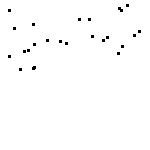
\includegraphics[width=0.3\textwidth]{figures/04_25_s_nocost.png}}
       }        
       \caption{Figures (a)-(c) show 3 out of 60 random instances for experiments. The instances differ in number and size of obstacles and are used for local costmap creation.}
      \label{fig:fig_instances}
   \end{figure}
   
\begin{figure}[thpb]
     \footnotesize
      \centering
      \setlength\fboxsep{0pt}
      \setlength\fboxrule{0.5pt}
       \def\svgwidth{\textwidth}
       %\fbox{\includesvg{figures/fig_inst_25_new}}
       \includesvg{figures/fig_inst_25_new}
		\caption[Local-path planning simulation.]{This figure shows three applications of the local planner in a simulated experiment. The greyscale background image visualizes obstacle costs of a generated costmap. Trajectories in green are drive-able, whereas red trajectories collide with obstacles. In each local planning step possible trajectories are weighted with respect to obstacle closeness and progression towards goal destination. For example in the second step a longer valid trajectory is rejected, while a shorter trajectory which stays farther away from obstacles is selected for execution. After three local planning applications the robot safely reaches the goal destination.}
		\label{fig:fig_instances_detail}
\end{figure}

The following list shows the tested algorithm:
\begin{itemize}
\item{\bf{Random Search with Tabu List:}} A repeated random guess of a velocity tuple $(v,w)$ (RST).
\item{\bf{Iterated Local Search:}} Performing Iterated Local Search with 4, 8 ,and 16 neighbors and Tabu List (ILS4, ILS8, ILS16).
\item{\bf{Variable Neighborhood Search:}} Variable Neighborhood search with Best-,and First-Improvement heuristic, and Tabu List (VNSB, VNSF).
\end{itemize}

\section{Test results}\label{sec:testresults}
All tests were performed on a 2.4 GHz, Intel Core 2 Duo processor using 4 GB RAM. 

In the first experiment the algorithms were applied to all 60 instances to evaluate a broad spectrum of possible environments. 
Figure~\ref{fig:fig_allworlds} illustrates the results using 240 trajectories, and using 2400 trajectory samples.
   \begin{figure}[thpb]
        \footnotesize
      \centering
      \def\svgwidth{0.7\textwidth}
      \includesvg{figures/fig_allworlds}
      \caption{This figure shows the results of testing all 60 randomly generated instances. The top figure shows the run time performance for 240 trajectories, and the bottom figure for 2400 trajectories. Compared to brute force search, the Meta-Heuristic algorithms show a significant improvement. }
      \label{fig:fig_allworlds}
   \end{figure}

 
The results show that all algorithms, including RST, outperform the Brute Force generate-and-test method significantly. 
As expected increasing the number of trajectories greatly favors the Meta-Heuristic algorithms, since they benefit from larger search spaces. 
Notice that ILS and VNS algorithms differ apparently from the RST by exhibiting much smaller variance in their test results, indicating that randomization alone is not enough to achieve very good and stable performance.
Furthermore the VNS exhibit a more stable performance than the ILS methods. 
Comparing the ILS algorithms reveals the connection of the search space size to the size of the neighborhood. 
A small number of trajectories benefits smaller sized neighborhoods, whereas increasing the number of trajectories benefits larger neighborhoods. 

The following tests only include the VNSF, VNSB and ILS4 algorithms. 
The algorithms are executed with specific world instances, and repeated 50 times. 
The results in Figure~\ref{fig:fig_special} show again that the VNS algorithms significantly outperform the Brute Force method. 

\begin{figure}[thb]
   \myfloatalign
   %\captionsetup[subfigure]{labelformat=empty} 
    \subfloat[]
    {  
       \def\svgwidth{\textwidth}
       \includesvg{figures/fig_6_40}
    }\\
    \subfloat[]
    {  
       \def\svgwidth{\textwidth}
       \includesvg{figures/fig_12_80}
    }
    \caption[Experiment: Trajectory size comparison]{The results of 50 consecutively executions with (a) 240 and (b) 960 trajectories, on particular instances which differ in number and size of obstacles. The blue line marks the run time for brute force search, which is used as a benchmark.}  
     \label{fig:fig_special}
\end{figure}
   
Analyzing the results of the ILS4 algorithms shows that a too small environment will quickly degrade to random search. 
Here the use of a neighborhood structure pays off and the VNS approaches perform evidently better than ILS. 
In addition, the results show that the algorithms perform good independent of number and size of obstacles.

As for nearly all optimization problems, the No Free Lunch theorems \cite{wolpert1997no} apply to the local planning domain. 
Looking at all the results, there is no clear winner among the algorithms. 
Nevertheless using Variable Neighborhood search with Tabu List and Best Improvement heuristic seem to yields the best and most stable overall performance. 

In general the run time of the python implementation is not very efficient compared to tuned C++ implementations. 
Therefore the absolute numbers of the run time evaluations should be handled with care. 

%\addtocontents{toc}{\protect\clearpage} % <--- just debug stuff, ignore
%\include{multiToC} % <--- just debug stuff, ignore for your documents
% ********************************************************************
% Backmatter
%*******************************************************
\appendix
\cleardoublepage
%\part{Appendix}
%%********************************************************************
% Appendix
%*******************************************************
% If problems with the headers: get headings in appendix etc. right
%\markboth{\spacedlowsmallcaps{Appendix}}{\spacedlowsmallcaps{Appendix}}
\chapter{Appendix Test}
Lorem ipsum at nusquam appellantur his, ut eos erant homero
concludaturque. Albucius appellantur deterruisset id eam, vivendum
partiendo dissentiet ei ius. Vis melius facilisis ea, sea id convenire
referrentur, takimata adolescens ex duo. Ei harum argumentum per. Eam
vidit exerci appetere ad, ut vel zzril intellegam interpretaris.

Errem omnium ea per, pro congue populo ornatus cu, ex qui dicant
nemore melius. No pri diam iriure euismod. Graecis eleifend
appellantur quo id. Id corpora inimicus nam, facer nonummy ne pro,
kasd repudiandae ei mei. Mea menandri mediocrem dissentiet cu, ex
nominati imperdiet nec, sea odio duis vocent ei. Tempor everti
appareat cu ius, ridens audiam an qui, aliquid admodum conceptam ne
qui. Vis ea melius nostrum, mel alienum euripidis eu.

\section{Appendix Section Test}
Ei choro aeterno antiopam mea, labitur bonorum pri no. His no decore
nemore graecis. In eos meis nominavi, liber soluta vim cu. Sea commune
suavitate interpretaris eu, vix eu libris efficiantur.

\graffito{More dummy text.}
Nulla fastidii ea ius, exerci suscipit instructior te nam, in ullum
postulant quo. Congue quaestio philosophia his at, sea odio autem
vulputate ex. Cu usu mucius iisque voluptua. Sit maiorum propriae at,
ea cum primis intellegat. Hinc cotidieque reprehendunt eu nec. Autem
timeam deleniti usu id, in nec nibh altera.

\section{Another Appendix Section Test}
Equidem detraxit cu nam, vix eu delenit periculis. Eos ut vero
constituto, no vidit propriae complectitur sea. Diceret nonummy in
has, no qui eligendi recteque consetetur. Mel eu dictas suscipiantur,
et sed placerat oporteat. At ipsum electram mei, ad aeque atomorum
mea.

\begin{table}
    \myfloatalign
  \begin{tabularx}{\textwidth}{Xll} \toprule
    \tableheadline{labitur bonorum pri no} & \tableheadline{que vista}
    & \tableheadline{human} \\ \midrule
    fastidii ea ius & germano &  demonstratea \\
    suscipit instructior & titulo & personas \\
    %postulant quo & westeuropee & sanctificatec \\
    \midrule
    quaestio philosophia & facto & demonstrated \\
    %autem vulputate ex & parola & romanic \\
    %usu mucius iisque & studio & sanctificatef \\
    \bottomrule
  \end{tabularx}
  \caption[Autem usu id]{Autem usu id.}
  \label{tab:moreexample}
\end{table}

Ei solet nemore consectetuer nam. Ad eam porro impetus, te choro omnes
evertitur mel. Molestie conclusionemque vel at, no qui omittam
expetenda efficiendi. Eu quo nobis offendit, verterem scriptorem ne
vix.

  
\begin{lstlisting}[float,caption=A floating example]
for i:=maxint to 0 do
begin
{ do nothing }
end;
\end{lstlisting}
%********************************************************************
% Other Stuff in the Back
%*******************************************************
\cleardoublepage%********************************************************************
% Bibliography
%*******************************************************
% work-around to have small caps also here in the headline
\manualmark
\markboth{\spacedlowsmallcaps{\bibname}}{\spacedlowsmallcaps{\bibname}} % work-around to have small caps also
%\phantomsection 
\refstepcounter{dummy}
\addtocontents{toc}{\protect\vspace{\beforebibskip}} % to have the bib a bit from the rest in the toc
\addcontentsline{toc}{chapter}{\tocEntry{\bibname}}
%\bibliographystyle{plainnat}
\bibliographystyle{plainnat}
\label{app:bibliography} 
\bibliography{Bibliography}

% ********************************************************************
% Game Over: Restore, Restart, or Quit?
%*******************************************************
\end{document}
% ********************************************************************
